% This is LLNCS.DEM the demonstration file of
% the LaTeX macro package from Springer-Verlag
% for Lecture Notes in Computer Science,
% version 2.3 for LaTeX2e
%
\documentclass[graybox]{svmult}

\usepackage{mathptmx}
\usepackage{helvet}
\usepackage{courier}
\usepackage{type1cm}

\usepackage{makeidx}
\usepackage{graphicx}

\usepackage{multicol}
\usepackage[bottom]{footmisc}

\usepackage{url}
\usepackage{color}
\usepackage{multirow}

\makeindex
%\newcommand{\XXXnote}[1]{{\bf\textcolor{red}{XXX: #1}}}
\newcommand{\XXXnote}[1]{{}}

\begin{document}

\title*{Volcano Monitoring : Addressing Data Quality\\Through Iterative Deployment}
\titlerunning{Volcano Monitoring}

\author{Geoffrey Werner Challen and Matt Welsh}

\institute{
Geoffrey Werner Challen \at Harvard School of Engineering and Applied Sciences,
\email{challen@eecs.harvard.edu}
\and Matt Welsh \at Harvard School of Engineering and Applied Sciences,
\email{mdw@eecs.harvard.edu}}

\maketitle

\abstract*{
Deploying wireless sensor networks to support geophysics presents an
interesting challenge. High data-rates required by geophysical
instrumentation preclude continuous data collection from even
moderately-sized networks. However, geoscientists are used to working
directly with complete signals, and therefor uncomfortable with in-network
processing that could reduce bandwidth by reporting data products.

Over five years of working with seismologists we have developed a lineage of
solutions driven by their scientific goals. Three field deployments have
provided valuable lessons and helped drive each successive design iteration.
We began by addressing datum quality, encompassing per-sample resolution,
accuracy, and time synchronization.  Later deployments focused on holistic
data quality, which requires considering constraints limiting full data
collection in order to maximize the value of the limited data retrieved. This
chapter uses our three deployments to demonstrate the benefits of iteration.
The first two illustrate our work on datum quality, while the last presents a
new approach to optimizing overall dataset quality.

}

\abstract{\newline
Deploying wireless sensor networks to support geophysics presents an
interesting challenge. High data-rates required by geophysical
instrumentation preclude continuous data collection from even
moderately-sized networks. However, geoscientists are used to working
directly with complete signals, and therefor uncomfortable with in-network
processing that could reduce bandwidth by reporting data products.

Over five years of working with seismologists we have developed a lineage of
solutions driven by their scientific goals. Three field deployments have
provided valuable lessons and helped drive each successive design iteration.
We began by addressing datum quality, encompassing per-sample resolution,
accuracy, and time synchronization.  Later deployments focused on holistic
data quality, which requires considering constraints limiting full data
collection in order to maximize the value of the limited data retrieved. This
chapter uses our three deployments to demonstrate the benefits of iteration.
The first two illustrate our work on datum quality, while the last presents a
new approach to optimizing overall dataset quality.

}

\newpage

% 18 Apr 2009 : GWA : Body of chapter.

\section{Introduction}
\label{sec-introduction}

Energy-harvesting sensor networks experience variations in load and charging
rates that threaten high-fidelity operation. Changing application demands can
produce variations in load rates, while energy-harvesting properties can
produce variations in charging rates. Energy mismanagement
can lead to reduced fidelity, when nodes' batteries empty, or wasted energy,
when nodes harvest energy they cannot store.

Energy harvesting capabilities such as solar charging further complicate the
distributed energy management task. The energy collected at each node may
vary significantly based on node placement, and the energy collected
day-to-day may vary significantly based on weather patterns. Preparing the
network for overnight operation requires capturing as much energy as possible
during the day and minimizing energy wasted by charging full batteries, while
overnight operation itself requires adjusting the network's load profile to
match the distribution of energy stored during daytime.

Fortunately, dense networks provide redundancy that can be used to control
the distribution of energy usage.  Multiple possible routing paths may
connect a node to the sink. Tuning MAC parameters allows nodes to shift
communication load to their neighbors. Sensor inputs from multiple nodes may
be redundant, allowing some to be disabled or operated at reduced fidelity.
The existence of these choices implies that it is possible to tune the energy
load of the network to better match energy availability.  Effective load
tuning can increase the fidelity provided to the application at a fixed
battery size, or allow battery sizes to be reduced while maintaining the
required fidelity level.

Existing sensor network platforms provide little support for collaborative
energy management. Approaches such TinyOS~\cite{tinyos-asplos00},
Pixie~\cite{pixie-sensys08}, Eon~\cite{eon-sensys07} and
Levels~\cite{levels-sensys07} facilitate local control only, failing when
greedy node energy minimization fails to produce the best outcome.
Network-wide solutions such as Lance~\cite{lance-sensys08},
Mercury~\cite{parkinsons-embs07}, and EnviroMic~\cite{enviromic} either
require centralized control or are tailored to the needs of a specific
application domain. In sensor networks the majority of energy consumption is
consumed by multi-node collaboration. We argue that due to the distributed
nature of energy consumption and availability, improving performance
requires consideration of both \textit{where} energy is and \textit{how much}
is being used.

Matching load to availability across the network requires \emph{integrating}
with application components producing energy load, \emph{distributing}
load and availability information to facilitate node decision making, and
\emph{awareness} of the connection between load, availability, and
application-level fidelity. We propose Integrated Distributed Energy
Awareness (IDEA), a sensor network service addressing these goals. IDEA
monitors and models the load and charge rates on each node.  To allow nodes
to reason about their impact on others, each node distributes its model
parameters, updating them as necessary to ensure continued accuracy.  IDEA
clients are responsible for estimating their own distributed energy
impact. When changing state, IDEA helps them evaluate each
proposed option using an energy objective function tailored to meet
specific application goals. By tracking availability and informing the energy
decision-making process, IDEA simplifies the construction of energy-aware
components.

Our paper makes the following contributions. First, we describe IDEA, a new
service uniting energy monitoring, load modeling and distributed state
sharing into a single service facilitating distributed decision making.
Second, we present three case studies illustrating how to use IDEA, including
a component that tunes MAC parameters, an existing routing protocol modified
to choose energy-aware routes, and a application using IDEA to determine how
to localize acoustic events.  Third, using simulation and testbed results we
compare the performance of IDEA with approaches that do not consider energy
distribution, showing that IDEA enables improvements in lifetime of up to
35\%.

The rest of this paper is organized as follows. Section~\ref{sec-motivation}
motivates the need for IDEA using a simple example. In
Section~\ref{sec-architecture} we present the IDEA architecture in detail and
describe our current implementation. We describe our three case studies in
detail in Section~\ref{sec-casestudies}. Section~\ref{sec-evaluation}
presents simulation and testbed results. We review related work in
Section~\ref{sec-related}, and Section~\ref{sec-futurework} outlines future
work and concludes.

\subsection{Datum v Dataset Quality}
\label{sec-datavdatumquality}

Reviewing our previous work, we have found it useful to divide our focus on
data quality into two separate concerns, \textit{datum} quality and
\textit{dataset} quality.  The former encompasses the quality of any one data
point, and requires addressing sampling rates, resolution, fidelity, and
accurate timestamping. Datum quality does not consider broader measures such
as the value of the data to the application, coverage or latency.  Such
higher-level metrics are incorporated in the idea of \textit{dataset}
quality, which considers the entire corpus of data presented to the
application or end user. This distinction is important because each requires
separate techniques to address.

Placed in this context, our first two deployments served to push the datum
quality to a level acceptable to the domain scientists.  Through the
experience that came with iteration, at the end we were able to convince
ourselves that we had built a system capable of meeting the science
\textit{datum quality} goals~\cite{volcano-osdi06}. Because the
application we chose happened to have fairly well-established datum quality
requirements, this work was iterating towards a fixed target.

Our interest in dataset quality reflects the inherent limitations of sensor
network devices.  Due to storage, bandwidth or power limitations, at some
point as the size of the network grows or the target lifetime increases, it
becomes infeasible to collect all signals from all nodes during the entire
deployment.  Thus the question emerges: what data should be collected in real
time and what data should not?  If the network is provisioned with adequate
storage and the deployment is of fixed length, data not delivered in
real-time may be eventually recovered manually; otherwise it will be lost.

Return a partial dataset to the end user also requires sorting the wheat from
the chaff.  Either some of the data has to be interesting enough to justify
eliding a great deal of the rest, or some of the data has to be uninteresting
enough to justify dropping it entirely.  Our application, volcano monitoring,
falls more into the first category, since seismologists would never concede
that any piece of signal is, prima facie, uninteresting. However,
they do have metrics allowing the value of a signal to be estimated and
compared against others, which allows system resources to be directed at the
most valuable signals.  Because seismological applications may benefit
sufficiently from the increased network resolution made possible by small,
low-power sensors, the discarded data that these networks imply is tolerable.

The high sample rates and per-sample resolution of seismic signals meant that
it only took a medium-size network to make full-signal streaming data
collection infeasible.  Given that the problem worsens as the network size
grows and target lifetimes increase, and our long-term goal is to deploy a
perpetually-powered network of several hundred nodes --- an order of
magnitude larger than any of our efforts to date --- addressing this problem
remains central to our ongoing research.

\subsection{Structure of this Chapter}

We begin by describing the key changes made between our initial deployment at
Tungurahua Volcano in 2004 and our second more significant effort at
Reventador Volcano in 2005.  Between these two deployments we made a large
number of changes addressing both datum quality --- including hardware board
development and time synchronization rectification --- and dataset quality
--- including reliable transport and event-driven data collection. We discuss
iterative improvements to the interface board and time synchronization in
Sects.~\ref{subsec-signalhardware} and \ref{subsec-multihoptimesync} below,
and outline the event triggered approach in Sect.~\ref{subsec-eventdriven}.

After beginning to address the datum quality requirements, we focused on
developing techniques that would advance the science goals by allowing the
size of the network or the duration of our deployments to be increased. This
meant addressing the dataset quality component. Our research in this area has
been a great deal more speculative since our seismologists are not used to
working with incomplete data sets, and while some of the flaws in earlier
systems drove our initial research direction, work in this area became
largely driven by the constraints inherent in wireless sensor network nodes:
storage, bandwidth, and power. Our work in this area culminated in
Lance~\cite{lance-sensys08}, an architectural framework for optimizing
dataset quality in the presence of constraints such as storage, bandwidth and
energy. Sections \ref{sec-prioritylance} and \ref{sec-utilitylance} describe
successive iterations of this framework, which emerged as part of our third
deployment in 2007, while Sect.~\ref{sec-policymodules} describes the
policy module component common to both.

Finally, addressing either datum or dataset quality in isolation, even while
holding one of them fixed, does not address overall data quality or
application-driven quality metrics.  Collected data is expected to be put to
use in service of some broader scientific goal, which likely has complex data
quality requirements not easily distilled into separate datum and dataset
goals.  We outline future directions intended to bridge this gap and conclude
in Sect.~\ref{sec-conclusions}.

\section{Sensor Interface Board}
\label{sec-sensorinterfaceboard}
\label{subsec-signalhardware}

\begin{figure}[t] 
\begin{center} 
\includegraphics[width=0.9\hsize]{./figs/EWSN2005/2005-VolcanoMote.eps}
\end{center} 
\caption{{\bf 2004 Volcano Mote.}
A Mica2 mote with simple sensor interface board allowing a single microphone
to be attached as shown.}
\label{fig-2004volcanomote}
\end{figure}

Of any system component, the hardware interface board received the most
significant internal redesign on the way to our second deployment in 2005.
Our proof-of-concept deployment deployed nodes fitted with a simple hardware
interface board interfacing the Mica2 motes at use at the time with a single
microphone.  The Mica2's 10~bit ADCs were used to collect acoustic signals at
100~Hz, the sampling rate necessary to capture volcanic infrasound.  Sampling
was driven by the Mica2's onboard oscillator and the standard TinyOS
\texttt{Timer} component. Figure~\ref{fig-2004volcanomote} shows a Mica2 mote
with the hardware interface board attached.

In particular, the following set of limitations of the original board had to
be addressed in order to provide the datum quality required by the
scientists:

\begin{enumerate}
\item {\bf Resolution:} Scientific analysis required a per-sample resolution
of at least 16~bits, with greater than 20 being ideal. The Mica2 motes used
for the original deployment provided only 10~bits of resolution and later
designs, such as the TelosB, provided only 16.
\item {\bf Filtering:} The ideal filter for the seismic and infrasonic data
our nodes were collecting is a hard cutoff at 50~Hz. Unfortunately, upon
review the original sampling board had a passive filter with a 3~dB point of
5~Hz which meant that desirable components of the signal were being
attenuated.
\item {\bf Number of Channels:} Fitting each node with both seismometers and
microphones, as we wanted to do for the second deployment, required allowing
multiple sensors to be attached to each node. Our original board was built to
interface a single sensor.
\item {\bf Timing:} We expected that providing the high-fidelity timing
necessary to track fast-moving pressure waves across the network would
require both a stable timing source driving the per-node sampling and a way
of interpreting local times across multiple nodes.  Multi-hop time
synchronization is discussed separately below, but the timing process
necessitated a stable local source that would produce clean per-sample
intervals.
\item {\bf Isolation:} When testing our Tungurahua deployment before fielding
it we noticed that, due to poor isolation between multiple chips on the
Mica2, radio transmissions were interfering with signal collection. The large
amount of current required to drive the CC1000 radio was flooding the ground
plane and causing the onboard ADC voltage reference to shift. While our
original system worked around this crudely in software, providing clean data
for scientists would require isolating the sampling components from sources
of potential interference.
\end{enumerate}

\subsection{2005 Board Redesign}
\label{sec-2005-board}

\begin{figure}[t]
\begin{center}
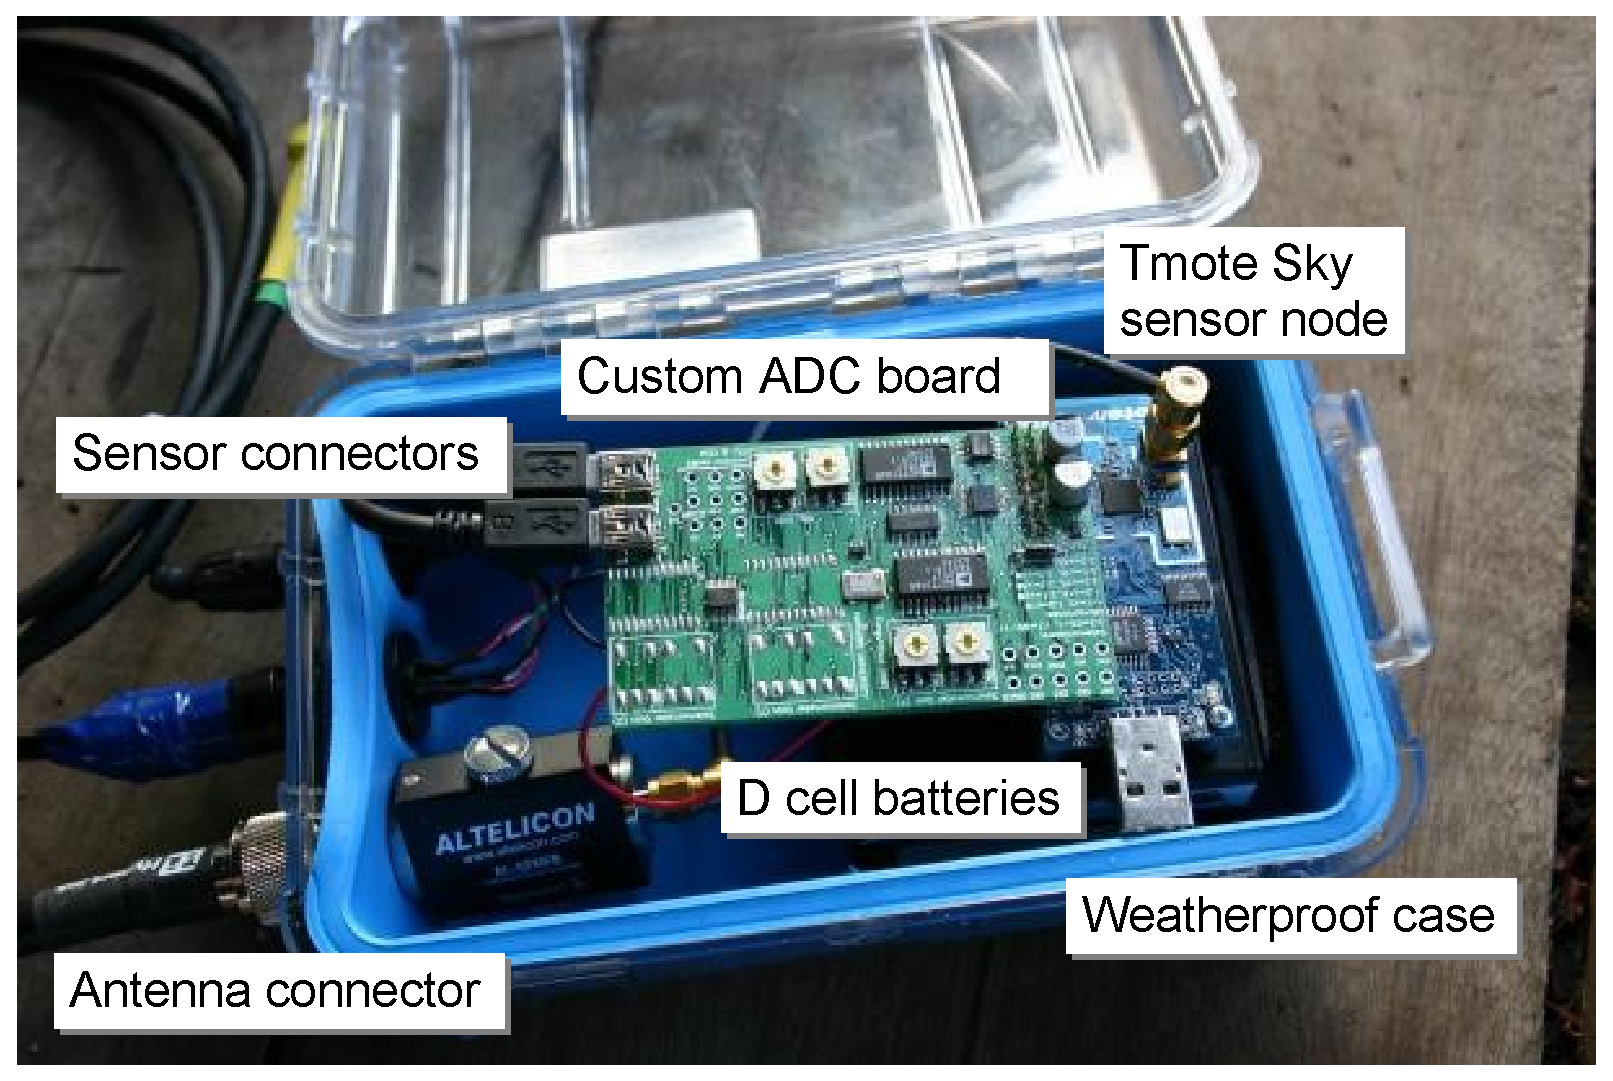
\includegraphics[width=1.0\hsize]{./figs/OSDI2006/2006-VolcanoMote.eps}
\end{center}
\caption{{\bf The second iteration of our volcano monitoring sensor
node, fielded at Reventador in 2005 and Tungurahua in 2007.}}
\label{fig-2005volcanomote}
\end{figure}

Initially, we considered using the TMote Sky's onboard ADCs.  The TMote had a
single 16~bit ADC --- which we believed to be well-isolated from other
circuitry on the node --- and the ability perform DMA sampling from the ADC
into onboard RAM while leaving the CPU in a low-power state.  However,
several limitations of the TMote led us towards a standalone board. First,
the 16~bit resolution of the onboard ADC was not quite enough to support our
application. Had this been the sole limitation we may have settled for
16~bits, but a separate board meant we could select higher-resolution ADCs.
In addition, the TMote had a \textit{single} 16~bit ADC, and we were worried
about multiplexing this between multiple channels.  Second, we were concerned
with providing a stable filter centered at 50~Hz.  Building a passive filter
at that low of a frequency is difficult, so we concluded that the filtering
would have to be done by an oversampling ADC.  Performing the filtering on
the TMote would have required oversampling at rates it was not capable of.

For these reasons we moved to a standalone sensor interface board providing
its own reference voltage (ensuring isolation), ADCs (allowing us to choose
the resolution and number of channels and implement digital filtering), and
clock source (ensuring a highly-accurate sampling rate).  Offloading this
much functionality to a hardware board was risky since it left us little room
for error in the design and fabrication, but it significantly simplified the
code running on the nodes themselves.  As it turned out, the fully
built-out application we deployed at Reventador Volcano consumed almost all
of the TMote Sky's 48~kB of program memory, leaving little room for the
functions we offloaded to the interface board.

As deployed in 2005 we were quite happy with the performance of our external
sensor interface board. The analysis conducted and reported
here~\cite{volcano-osdi06} showed no significant deficiencies in the board
design.  There was some initial confusion about the sampling rate which, due
to the precision of the oscillator and the settings on the ADC, turned out to
be slightly less than exactly 100.000~Hz, but it was extremely consistent
across multiple nodes meaning that data collected from several stations could
be lined up and processed together.  We designed software allowing us to
modify the ADC settings on-the-fly and this came in handy during the
deployment when we realized that the hardware gain settings were too low. We
were able to modify them in software and address the problem without
returning to the deployment site.

%\subsection{Interfacing to the TMote Sky}
%
%Once we chose to fabricate our own board several other questions emerged.
%First, how would we interface our board to the TMote itself?  Second, how
%configurable did we want the sensor interface board to be?
%
%The first question we resolved in favor of choosing ADCs featuring a simple
%serial interface that could be manually-clocked (i.e. ``bit banged'') to
%clock out samples.  While a high-speed bus such as SPI or I2C would have
%greatly sped up the communication between node and board, we were concerned
%about arbitrating the multiple devices sharing these buses already and chose
%to further separate our hardware board onto its own dedicated communication
%lines. This decision, however, led to a tradeoff in terms of the
%configurability of the device, since we were limited by the number of
%available pins on the headers exposed by the TMote Sky.  By using all
%available externally-exposed pins we were able to operate and configure the
%external ADCs, but the small number of pins led to the exclusion of some
%seemingly obvious functionality. For example, there was no way to turn the
%entire sampling board on or off, which a more intelligent node might have
%wanted to do to save power, or to reset the sampling board components to a
%known good state. Additionally, due to an overlap between two pins
%configuration settings on the ADCs --- such as the sampling rate and internal
%gain --- could be written, but not read.
%
%As far as configurability the ADC that we chose exposed a number of different
%settings that we found useful. In particular, in the field we used the
%internal gain setting on the ADCs to work around a poor choice of hardware
%gain settings on the hardware board itself. Hardware gain settings, which
%could be controlled through rotational switches, were another element of
%configurability we included on the board itself.  Unfortunately, as it
%happened local testing using the seismometers and microphones we deployed led
%us to choose an overly insensitive set of gain settings to canonicize on the
%board itself. When the system was fielded and collected data showed the
%hardware gain settings, even at their highest, to be too low, we were able to
%change the ADC's internal gain using a software command.  Because changing
%the internal gain damaged the effective resolution of the ADC, we were happy
%at that point to have deployed an ADC wider than what was strictly necessary.
%The ADCs also included a number of different configuration parameters that,
%while potentially useful, we never explored, such as the ability to change
%the sampling rate.


\subsection{Performance and Future Designs}

The external interface board was not without its drawbacks. In particular,
the oversampling ADCs we chose consumed a large amount of power, around 8~mA
per ADC.  When combined with other board components, such as the reference
voltage, 3 to 5V conversion necessary to power certain components, and
external oscillator, the sensor interface board ended up consuming around
60~mA of current, or around 3 times more than the TMote with radio and CPU
fully active.  As mentioned previously, there is no way to power down the
interface board remotely, nor would we be able to without immediately losing
data since the ADCs are sampling at tens of kHz.  For the Reventador
deployment we provisioned around this high power consumption by deploying
larger (D~cell) batteries and replacing them several times.  This can be seen
as a tradeoff between datum quality --- which necessitates the high-power
external sensor interface board --- and a reduction in dataset quality
through shorter systems lifetimes or higher-duty cycles due to increased
power consumption.

It is likely that the next iteration of this board will take on several
additional challenges. First, we will strive to lower the power consumption
while maintaining high fidelity through the use of newer ADCs which can hold
down their current consumption even while performing the several factors of
oversampling necessary to perform digital filtering.  Second, we are
increasingly interested in the ability to support multiple applications.
Thus any future sensor board design, either built in-house or purchased
as-is, will be expected to support multiple applications and sensor types.
Our current board is, in its choice of ADCs and hardware-filtering,
somewhat tailored to the volcano application. We'd like to move away from
this if possible.

These two future goals are in many ways at odds with each other, since the
challenge of reducing the power consumption of a board designed for a very
specific purpose is different and potentially more manageable than the
challenge of designing a general-purpose yet low power board. This is a
design tension that we expect to continue to play out in future hardware
revisions.

\section{Time Synchronization}
\label{sec-timesynchronization}
\label{subsec-multihoptimesync}

Unlike the sensor interface board, in which a simple prototype led directly
to a more successful second effort, achieving high precision time
synchronization between nodes is a battle we have continued to fight through
multiple design iterations.  Indeed, at present we are not yet certain a
suitable solution has truly been found, or whether this challenge will
reemerge while preparing the next deployment.  The problem of accurate timing
is one shared by multiple applications and deployment efforts, and
significant effort has taken place in this area.

Accurate timestamping arises directly from the analysis performed on seismic
and infrasonic volcano data, with the required precision dependent on the
intended use and other aspects of datum quality such as the sampling rate.
Seismic signals can move across a deployed array at thousands of meters per
second, with acoustic signals moving at the speed of sound, (roughly
300~m/s). If two neighboring stations are deployed 100~m apart (possible with
good line of sight and powerful antennas) a seismic signal can cross that gap
in tens of milliseconds and an acoustic signal in hundreds of milliseconds. At
a typical seismological sampling rate of 100~Hz this means that seismic wave
arrival times at the two stations might only differ by one or two samples,
necessitating precise time synchronization if the propagation of these waves
is to be accurately captured.  Thus our target accuracy for timestamping has
typically been 10~milliseconds: a single sample interval.

Wired seismic instrumentation frequently deploys a single GPS receiver at
each station, with the power required to operate GPS-driven timestamping a
less significant component of the station's power budget. While we considered
this approach (as described below), we ultimately rejected it due to its
prohibitive power consumption.

\subsection{Single-Hop Time Synchronization}

Our first deployed system made use of a simple time synchronization approach
appropriate in a single-hop environment.  A single node was attached to a
Garmin GPS ``puck'', which provides a highly-accurate (within 1~microsecond)
pulse-per second output. This was trapped by an interrupt pin and, when
triggered, that node sent out a broadcast radio message that should reach all
other nodes. Upon receiving the message, each sampling node marked the sample
that it was in the process of collecting as occurring at that moment in time.
Beginning with this mapping between some of the samples (roughly one out of
every 100) and the GPS per-second pulse, an accurate timestamp can be
assigned to each sample via linear interpolation. (A more complete
description of this protocol is contained in
previously-published~\cite{volcano-ewsn05} work.)

This simple approach has many desirable properties, particularly when the two
enemies of time synchronization in wireless sensor networks --- skew and
drift --- are considered. Skew reflects the fact that all oscillators are not
created equal, and that two oscillators sold as identical will, in fact,
differ by some small amount. This is particularly true of the less expensive
crystals used on low-cost wireless sensor network nodes. Drift names the
tendency of the true rate of any particular oscillator to change over time,
due to environmental changes such as temperature and humidity.  Thus even if
two oscillators started out perfectly in synch changes to their local
environments would cause them to drift apart slowly over time. Because the
GPS PPS is guaranteed to be accurate and displays no drift, the accuracy of
the broadcast message rate can be guaranteed. And, even in the presence of
skew and drift on the receivers, as long as the drift rates are bounded the
interpolation between neighboring PPS signals should yield accurate results.
However, the single-hop approach obviously does not work in a multi-hop
environment where the multiple sampling nodes cannot all hear the GPS
broadcast.

\subsection{Adaptation to Multi-Hop Using FTSP}

During the three deployments we have performed, a single GPS node was
deployed near a large power source (car battery) that also powered other
pieces of critical infrastructure (the root of the spanning tree and
long-distance point-to-point serial communication linking the deployment site
to the volcano observatory).  Provisioning multiple GPS nodes with the power
necessary to enable acceptable system lifetimes would have greatly
increased our deployment burden, and so a software solution was sought.

We ended up deploying a new wireless sensor network protocol called FTSP
(Flooding Time-Synchronization Protocol)~\cite{ftsp}, which was released
around the time that we completed our deployment at Tungurahua.  FTSP allows
a network of nodes deployed into a multi-hop topology to share a single
global clock by providing mappings between a local timestamp on any node and
the global timebase. Our plan was to timestamp our data by performing two
mappings: the first would map the local time on each node into the global
FTSP time; the second would map the global FTSP time into the GPS time.  We
would rely on FTSP to perform the first mapping and deploy a single node with
GPS to allow us to perform the second.

\subsection{Observed FTSP Instabilities}

During the testing that preceded our 2005 deployment at Reventador a number
of problems were seen with FTSP in a lab setting. Sometimes the global time
would become wildly inaccurate for a period of time before settling back to
being quite accurate.  We were unable to track down the source of this
instability, although we did make multiple changes to the protocol in
attempts to harden it and tailor it for our particular application. However,
the faults we observed in the lab were all temporary in nature, and we
believed that although FTSP did not seem to be always accurate it was stable
and able to correct itself when it got off track.

The behavior we observed upon deploying the system was radically different.
We did see, periodically, the small, correctable bits of instability that we
had observed in the lab.  However, we also noticed longer stretches of
instability that seemed uncorrectable by FTSP itself.  The only solution to
rectify the timing on nodes that entered into this state was to reboot them,
which forced them to resync upon protocol restart.  While we eventually built
monitoring and automatic reboots into the system driver software running at
the base station, allowing automatic reboots of nodes with troubled timing,
the stretches of timing outages frustrated our attempts to collect clean,
well-timestamped data.

\begin{figure}[t]
\begin{center}
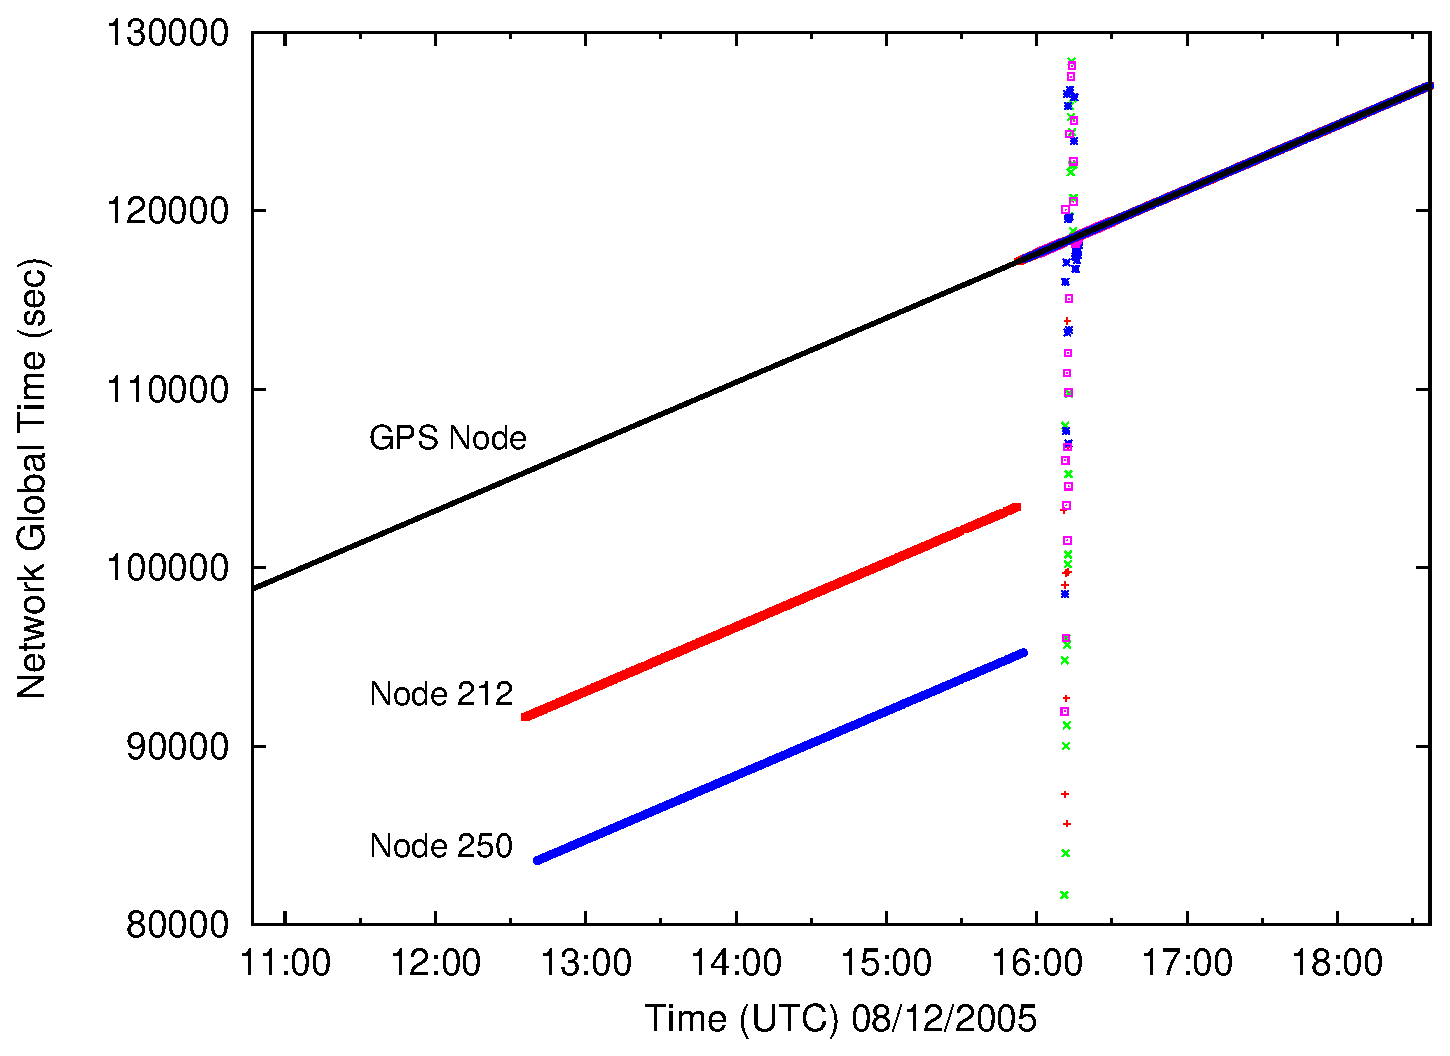
\includegraphics[width=\hsize]{./figs/OSDI2006/2006-FTSPInstability.eps}
\end{center} 
\caption{{\bf Example of FTSP instability observed during field deployment.}
The global time value reported by sensor nodes and the GPS node is plotted
against the time that the base station received the corresponding status
messages. All nodes are initially synchronized, but starting at 1230 GMT,
nodes 212~and~250 report incorrect global times for the next 4.5~hours. When
the nodes eventually resynchronize, the global timestamps of other nodes
initially experience some instability.}
\label{fig-FTSPInstability}
\end{figure}

Figure~\ref{fig-FTSPInstability} shows an example of the FTSP instability
observed in the field. The global time reported by two nodes suddenly jumps
off by several hours, and the nodes do not resynchronize until rebooted
4.5~hours later.  It turns out that two bugs combined to cause this problem.
First, it was discovered that the TinyOS clock driver would occasionally
return bogus local timestamps.\footnote{This bug was fixed in February 2006, several
months after our deployment.} Second, FTSP does not check the validity of
synchronization messages, so a node reading an incorrect value for its local
clock can corrupt the state of other nodes, throwing off the global time
calculation.

\begin{figure}[t]
\begin{center}
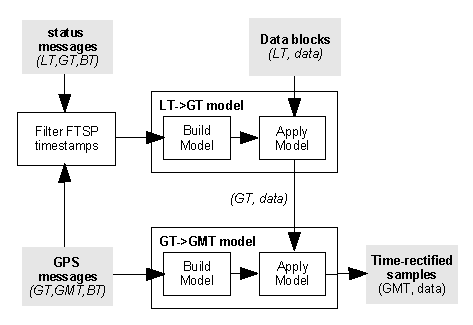
\includegraphics[width=0.8\hsize]{./figs/OSDI2006/2006-RectificationCartoon.eps}
\end{center}
\caption{{\bf Time rectification process overview.}}
\label{fig-rectificationcartoon}
\end{figure}

The failures of the time synchronization protocol made establishing the
correct GPS-based timestamp for each data sample extremely challenging.  To
do so, we developed a {\em time rectification} approach which filters and
remaps recorded timestamps to accurately recover timing despite these
failures. Figure~\ref{fig-rectificationcartoon} shows an overview of the
process.  The first step is to {\em filter} the global timestamps recorded
by each node, discarding bogus data. Second, we build a model mapping the
local time on each node to FTSP-based global time.  Third, we use the GPS
timestamp information to build a second model mapping FTSP time to GMT.
Finally, both models are applied to the timestamps recorded in each data
block producing a GMT time for each sample.

\subsubsection{Timestamp Filtering}
\label{subsection-filtering}

We begin by filtering out status messages appearing to contain incorrect
global timestamps. To do this, we correlate global timestamps from each node
against a common reference timebase and reject those that differ by more than
some threshold.  For this, we use the base station laptop's local time, which
is {\em only} used for filtering FTSP timestamps, not for establishing the
correct timing. The filtering process in is many ways similar to prior
work~\cite{paxson98calibrating,1028824} on detecting adjustments in
network-synchronized clocks.

We use the following abbreviations: {\em LT} is the local time of a node;
{\em GT} is the FTSP global time; {\em BT} is the base station's local time;
and {\em GMT} is the true GMT from the GPS signal.  The single GPS node
periodically sends a message logged by the base station consisting of the
triple {\em (GT, GMT, BT)}.  We use linear regression on this data to produce
a reference timebase mapping {\em BT} to {\em GT}.\footnote{We assume that
the global time reported by the GPS node is always correct; indeed, the
definition of ``global time'' is the FTSP time reported by the GPS node.}
Nodes periodically report their status through a heartbeat message, which
includes their local (LT) and global (GT) times, and for each node status
message logged by the laptop {\em (LT, GT, BT)}, we map {\em BT} to the
expected $\mathit{GT}_{\mathit{ref}}$ using the reference timebase. If $ \mid
\mathit{GT}_{\mathit{ref}} - \mathit{GT} \mid > \delta$, we discard the
status message from further consideration.  We use a threshold of $\delta =
1$~sec.  Although radio message propagation and delays on the base station
can affect the {\em BT} for each status message, a small rejection threshold
$\delta$ makes it unlikely that any truly incorrect FTSP timestamps pass the
filter. Indeed, of the 7.8\% of timestamps filtered out, the median {\em GT}
error was 8.1~hours.


\subsubsection{Timestamp Rectification}
\label{section-timerectification}

\begin{figure}[t]
\begin{center}
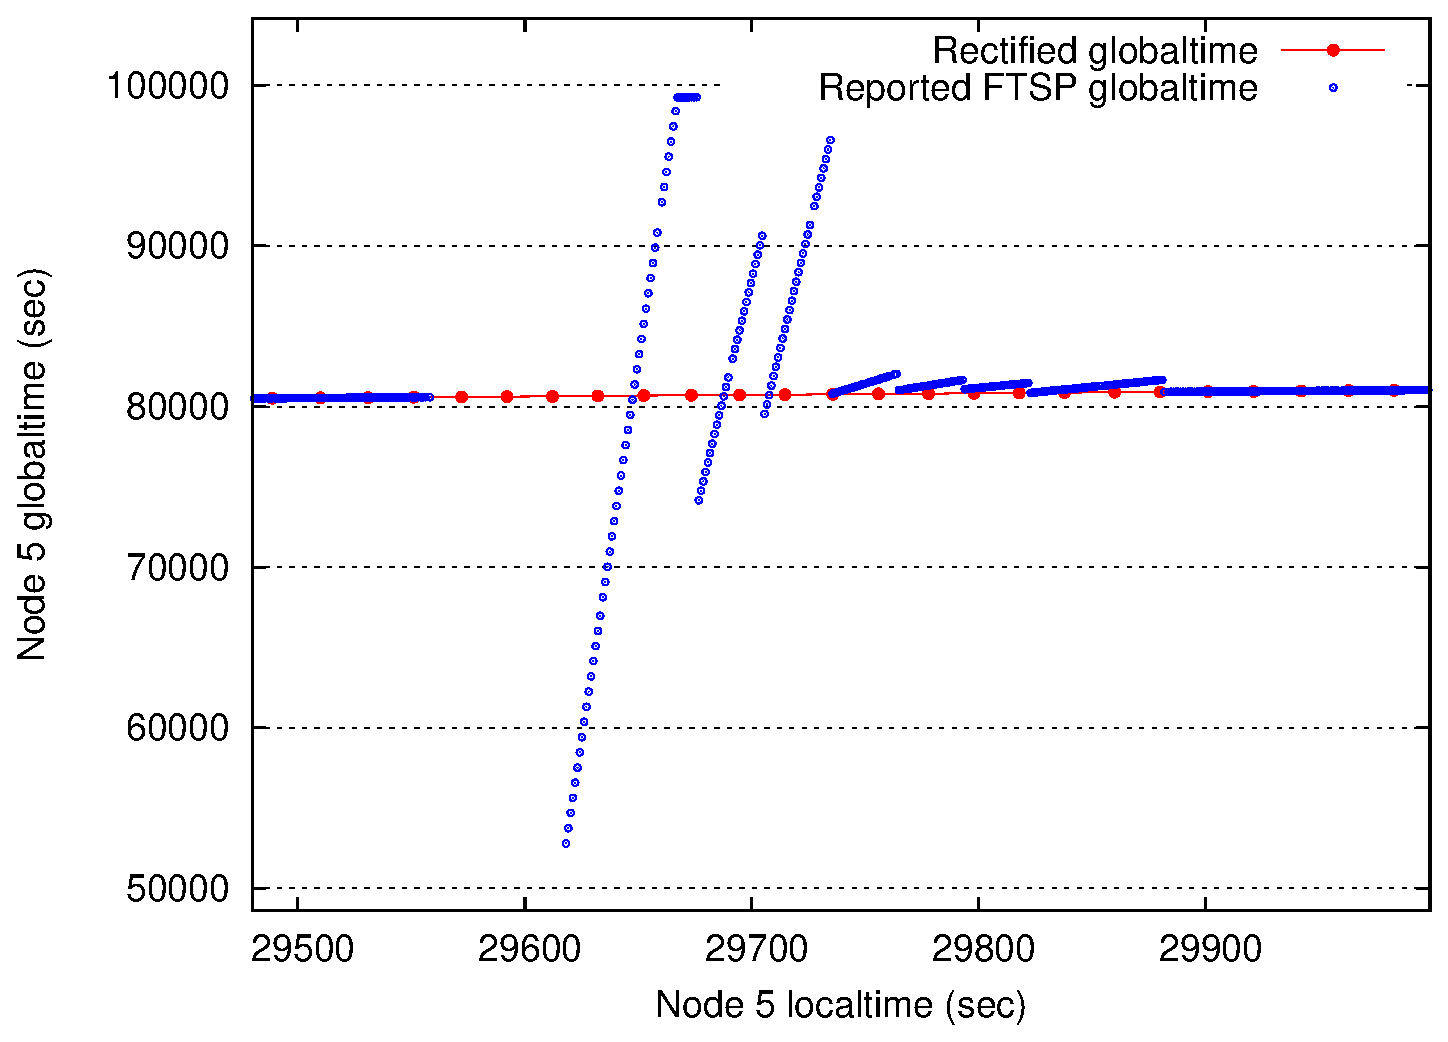
\includegraphics[width=\hsize]{./figs/OSDI2006/2006-TimingRectificationExample.eps}
\end{center}
\caption{{\bf Time rectification example.}
The raw (LT, GT) pairs collected from the node show that it experiences a
period of FTSP instability.  The time rectification process removes the
errant timestamps creating an accurate mapping between LT and GT created
using a linear regression on the remaining timestamps.}
\label{fig-timingrectificationexample}
\end{figure}

The goal of {\em time rectification} is to assign a GMT timestamp to each
sample in the recorded data. In order to do so, we build two models: one
mapping a node's local time to global time, and another mapping global time
to GMT. Figure~\ref{fig-timingrectificationexample} shows an example of this
process bridging a small local timing instability of the kind described
previously.

From those status messages that pass the filter, we build a piecewise linear
model mapping {\em LT} to {\em GT} using a series of linear regressions.
Models are constructed for each node separately, since local times vary
significantly between nodes.  Each regression spans up to 5~minutes of data
and we initiate a new regression if the gap between subsequent {\em (LT, GT)}
pairs exceeds 5~minutes.  Each interval must contain at least two valid
status messages to construct the model.  We take the {\em LT} value stored in
each data block and use this model to recover the corresponding {\em GT}
value.

The next step is to map global time to GMT. Each of the GPS node's status
messages contain a {\em (GT, GMT)} pair. As above, we build a piecewise
linear model mapping {\em GT} to {\em GMT}, and apply this model to the {\em
GT} values for each data block. Finally, we assign a GMT value to each sample
contained in the block, using linear interpolation between the GMT values
assigned to the first sample in each block.  This process makes no
assumptions about sampling rate, which varies slightly from node to node due
to clock drift.

\subsection{Evaluation}

Evaluating our time rectification process proved difficult, primarily because
we had no ground truth for the timing of the signals recorded in the field.
However, by reproducing the deployment conditions in the lab, we were able to
measure the accuracy of the recovered timing in a controlled setting.  In
addition, as described earlier, two GPS-synchronized data loggers were
colocated with our sensor network, providing us the opportunity to directly
compare our time-rectified signals with those recorded by conventional
instrumentation.

\subsubsection{Lab Experiments}

Our first validation took place in the lab. Feeding the output of a signal
generator to both a miniature version of our sensor network and to a
Reftek~130 data logger allowed us to directly compare the data between both
systems.  The miniature network consisted of a single sensor node, routing
gateway, and GPS receiver node. The same software was used as in the field
deployment. The Reftek~130 logs data to a flash memory card and timestamps
each sample using its own GPS receiver.

The results showed a consistent 15~ms offset between the time-rectified
signals recorded by the sensor node and the Reftek data logger.  We
discovered that this offset was due to delays introduced by the digital
filtering performed by the ADC on our sensor board (see
Sect.~\ref{sec-2005-board}). Adjusting for this delay resulted in an
indiscernible offset between the sensor node and Reftek signals. While this
experiment does not reproduce the full complexity of our deployed network, it
does serve as a baseline for validation.

In the second lab experiment, we set up a network of 7~sensor nodes in a
6-hop linear topology. The topology is enforced by software, but all nodes
are within radio range of each other, making it possible to stimulate all
nodes simultaneously with a radio message.  Each node samples data and sends
status messages using the same software as the field deployment. The FTSP
root node periodically transmits a beacon message. On reception of the
beacon, each node records the FTSP global timestamp of the message reception
time (note that reception of the beacon message is not limited by the
software-induced topology).  Because we expect all nodes to receive this
message at the same instant (modulo interrupt latency jitter) we expect the
FTSP time recorded at each node to be nearly identical. The FTSP root also
records the time that the beacon was transmitted, accounting for MAC delay.
The experiment ran for 34~hours, during which time FTSP experienced
instabilities similar to those seen during our deployment.

\begin{figure}
\caption{{\bf Timestamp errors in a 6-hop lab testbed.}
This table shows the 50th and 90th-percentile timing errors on both the raw
FTSP timestamps, and rectified timestamps.}
\vspace{0.2in}
\begin{center}
\begin{tabular}{lll}
\noalign{\smallskip}
                  & {\bf Raw error} & {\bf Rectified error} \\
\noalign{\smallskip}\svhline\noalign{\smallskip}
{\bf  1 hop}, 50th percentile & 1.52 ms & 1.42 ms \\ 
{\bf 1 hop}, 90th percentile & 9.86 ms & 6.77 ms \\
\noalign{\smallskip}\svhline\noalign{\smallskip}
{\bf 6 hops}, 50th percentile & 2.63 ms & 2.18 ms \\ 
{\bf 6 hops}, 90th percentile & 13.5 ms & 6.8 ms \\
\end{tabular}
\label{fig-time-rect-lab}
\end{center}
\end{figure}

This allows us to compare the {\em true} global time of each beacon message
transmission and the {\em apparent} global time on each receiving node, both
before and after subjecting the data to our time rectification process.  We
call the difference between the true and apparent times the {\em timestamp
error}. Figure~\ref{fig-time-rect-lab} shows the results for nodes one and
six hops away from the FTSP root.  After rectification, 99.9\% of the errors
for the one-hop node and 93.1\% of the errors for the six-hop node fall
within our 10~ms error envelope.

\subsubsection{Comparison with Broadband Station}

\begin{figure}[t]
\begin{center}
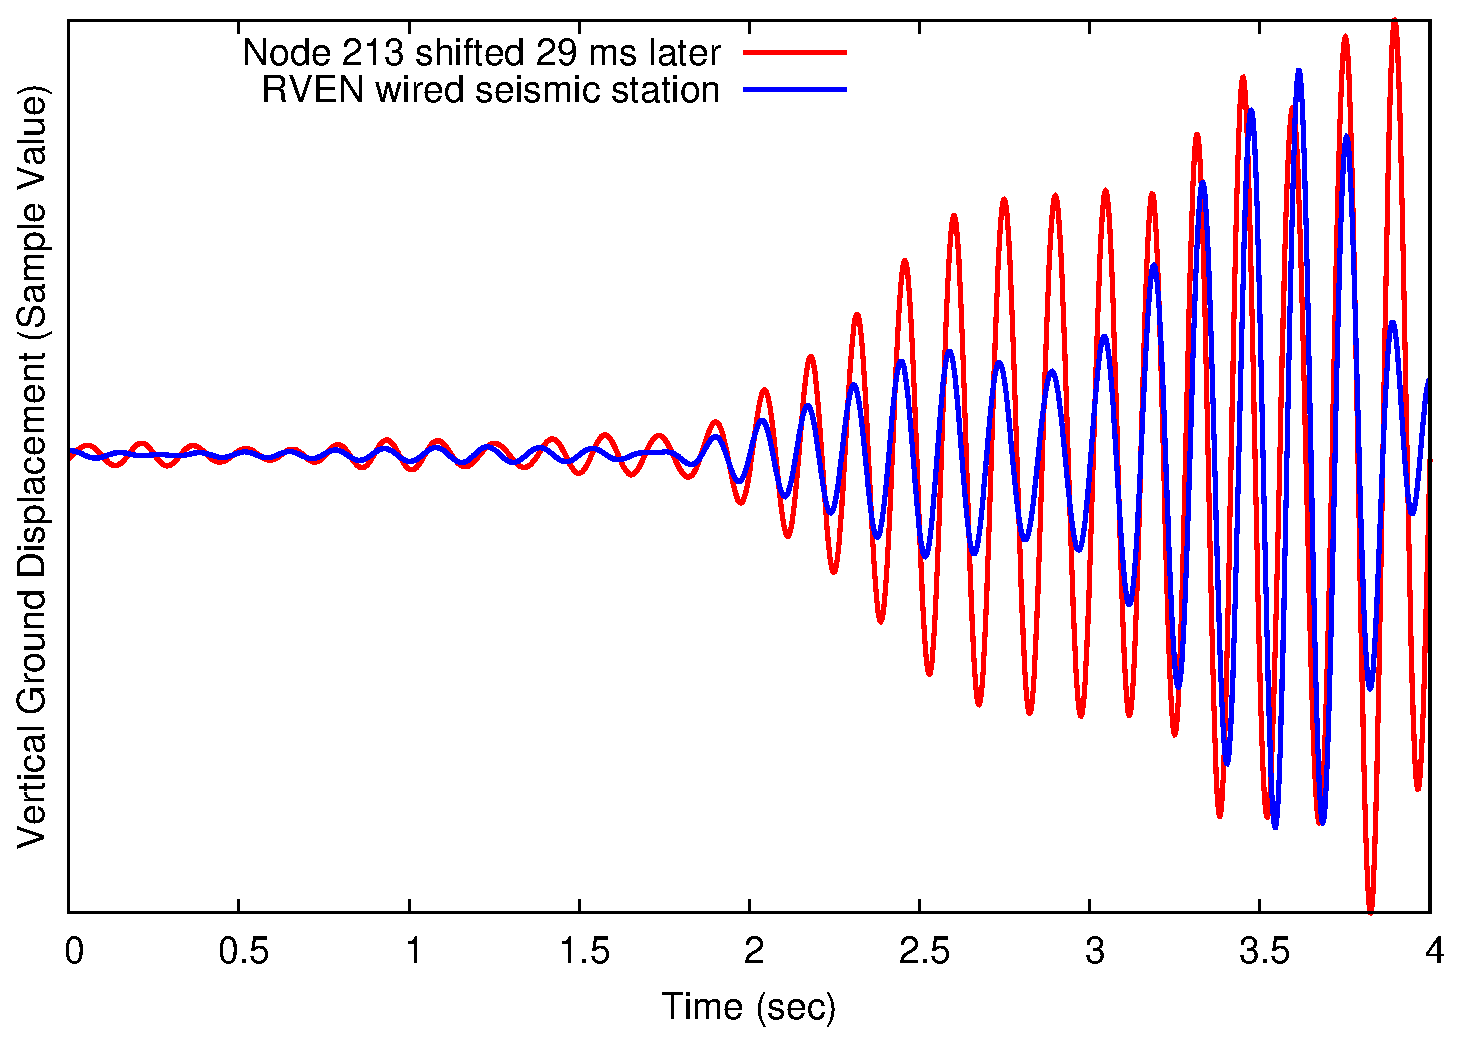
\includegraphics[width=\hsize]{./figs/OSDI2006/2006-reftekTimingExample.eps}
\end{center}
\caption{{\bf Comparison of RVEN and node~213 signals.}
This figure shows two seismic waves recorded by sensor node 213 and a
broadband seismometer located 56~m away. After time rectification, a 29~ms
time shift produces an excellent match.}
\label{fig-reftektimingexample}
\end{figure}

Although time rectification works well in the laboratory, it is also
necessary to evaluate its accuracy on the data collected during the field
deployment. For this purpose, we made use of one of the broadband seismometer
stations colocated with our sensor network. The RVEN (for ``Reventador
vent'') station was located 56~m from sensor node~213 (See
Fig.~\ref{fig-deployment-maps}(b)).  Given their
proximity, we would expect the seismic waveforms captured by both RVEN and
node~213 to be well correlated.  Some time shift between the two signals
would be expected: a seismic wave passing each station could be as slow as
1.5~km/sec, so the time lag between the signals could be as high as 37~ms.
However, due to differences in the seismometers and the placement and ground
coupling of the sensors, we would not expect perfectly correlated signals in
every case.

We identified 28~events recorded by both RVEN and node~213.  The data for
node~213 was time rectified as described earlier, and the RVEN data was
timestamped by the Reftek's internal GPS receiver.  We applied a bandpass
filter of 6--8~Hz to each signal to reduce sensor-specific artifacts. The
cross-correlation between the signals produces a set of of {\em lag times}
indicating possible time shifts between the two signals.  Due to the periodic
nature of the signals, this results in several lag times at multiples of the
dominant signal period. For each lag time, we visually inspected how well the
time-shifted signals overlapped and picked the best match by hand.

\begin{figure}[t]
\begin{center}
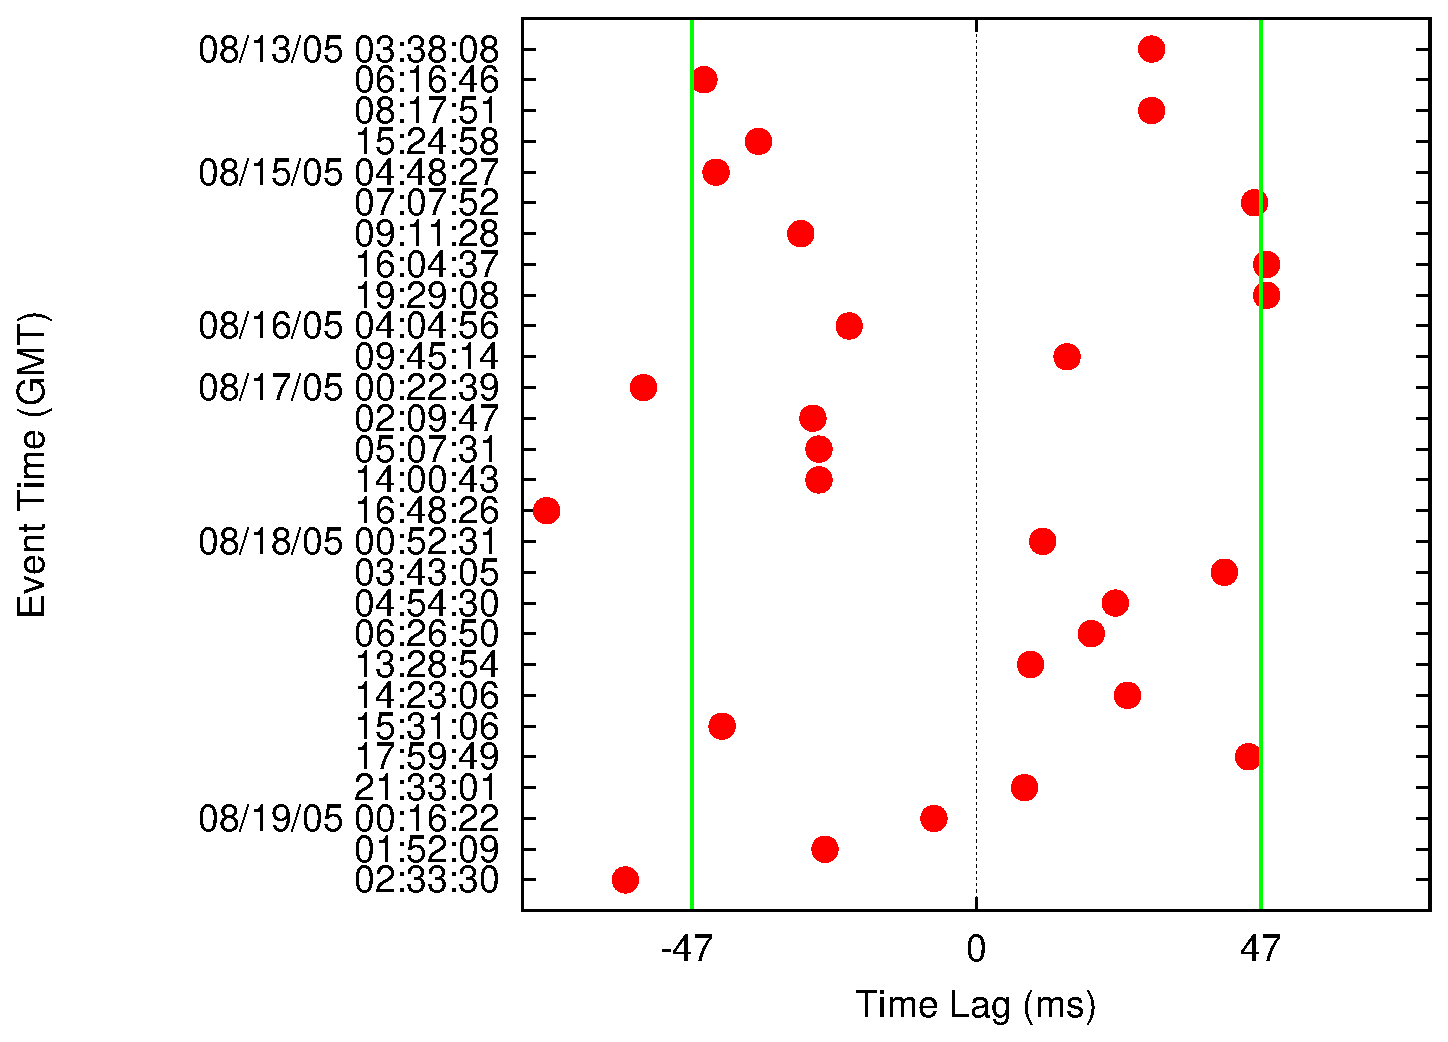
\includegraphics[width=\hsize]{./figs/OSDI2006/2006-TimingLags.eps}
\end{center}
\caption{{\bf Lag times between Node 213 and RVEN.}
The best lag time between the two stations is shown for 28 events.  best time
lag between the two stations is shown.  Most time shifts into the +/-~47~ms
window that we would expect given the distance between the two stations and
up to 10~ms of timing error.}
\label{fig-timinglags}
\end{figure}

Figure~\ref{fig-reftektimingexample} shows an example of this process that demonstrates
excellent correlation between the RVEN and node~213 signals with a 29~ms time
shift. Figure~\ref{fig-timinglags} shows a scatter plot of the best lag times
for all~28~events.  Of these, only 5~events fall outside of a $+/-$~47~ms
window defined by the distance between the stations ($+/-$~37~ms) and our
acceptable sampling error (10~ms). We have high confidence that our
time rectification process was able to recover accurate timing despite
failures of the FTSP protocol.

\subsection{Lessons Learned}

Overall there were many lessons we took away from our experience with data
timestamping.  First, due to the fact that development of the time
rectification technique took several months after the system teardown time,
we missed the critical window during which the scientific interest in our
data peaked.  Arriving in the field with an end-to-end solution ready to take
the output of our network and mold it into a form suitable for scientific
inspection would have been ideal, and is highly advisable for deployments
where scientist have clear datum quality expectations going in, as ours did.  

In addition to being unprepared for the issues we observed in the field, we
also did not think through the impacts of presenting half-baked data to the
seismologists we have been working with.  Particularly given our worries
about other parts of the system that did end up performing satisfactorily,
like the sampling board and driver (Sect.~\ref{subsec-signalhardware}), bulk
data transfer protocol and event detection mechanism, we were excited when
any signals at all showed up at the base station laptop. In our rush to
deploy the system we had not prepared an adequate data analysis and
visualization environment, and much of this was developed on-the-fly as the
deployment progressed. Due to this late and rushed development, none of the
initial tools did any of the post-hoc timing rectification that we eventually
had to perform in order to make the data suitable for scientific study.
Instead, we devised primitive tools allowing data from multiple stations to
be plotted together.

Unfortunately, these stacked plots were interpreted very differently
by the computer scientists and seismologists. To the computer scientists
these were evidence that the network was sampling data, detecting events and
successfully retrieving data using our bulk data-transfer protocol, namely
things were \textit{working}. Less concerned with the inner workings of our
system the seismologists appreciated little of this.  To them, these
poorly-synchronized signals were instead evidence that our signal timing was
extremely broken, a fear that persisted for some time after the deployment as
we worked hard together to rectify and validate the timestamps.  
The exposure of this intermediate data product to consumers unprepared for it
should serve as a cautionary tale about how much of the internal engineering
of a deployed WSN application to reveal externally.

Validating the timestamps on the data we did collect was also quite
frustrating and illustrates to what degree we were unprepared for the
severity of the timing challenge.  The several wired data loggers deployed
alongside our network all had attached GPS units providing extremely accurate
signal timing.  Had we thought to attach a single sensor both to one of our
wireless stations and, by simply splitting the output signal, to one of the
wired stations we could have easily cross-checked the timing with a known
ground truth (i.e. the identical signal).  In a remarkable oversight we never
thought to do this, meaning that we had no two identical inputs available to
reveal any inaccuracies in the timing information for the signals we
collected.  It would also have been useful to spend more time hardening FTSP
pre-deployment, and to have built in more logging and visibility into its
operation to help us at least have an idea, in situ, of how well it
was functioning.

While further work in this area would have been possible, our interests after
the 2005 deployment tended more in the direction of improving dataset
quality. Given our techniques to rectify the timestamps provided by FTSP were
already in place going forward, little additional work was done in this area.
In addition, FTSP has continued to be maintained and was canonicized as an
official mainline part of TinyOS in version 2.1.1 Given the importance of
accurate timestamping to many sensor network applications, certainly ones in
the scientific space, it is extremely encouraging that the sensor network
community has indicated its willingness to continue to test and maintain this
critical component.

\section{Event Triggering}
\label{sec-eventtriggering}
\label{subsec-eventdriven}

While our proof-of-concept deployment had each node attempting to stream a
continuous signal over a single radio hop to the base station, this approach
did not scale to more nodes deployed into a multi-hop topology.  In fact, it
didn't even work that well with the small number of nodes we deployed in
2004. Analysis of our data showed many dropouts and periods of missing data
caused by simple packet delivery failures. Some nodes were impacted more than
others, but all deployed nodes displayed this weakness.

Going into the 2005 deployment we knew that we needed a more scalable
approach. The one that we developed was, in its own way, a precursor to the
more intensive dataset work that would develop into a separate
data-collection framework.  What we decided to do was exploit the network's
monitoring capability to help decide what data was interesting, and capture
that data at the expense of other signals.

The way that this worked was as follows.  Nodes were programmed to locally
detect interesting seismic events and transmit event reports to the base
station. If enough nodes triggered in a short time interval, the base station
attempted to download the last 60~sec of data from each node.  The download
window of 60~sec was chosen to capture the bulk of the eruptive and
earthquake events, although many volcanic events can exceed this window
(sometimes lasting minutes or hours).  To validate our network against
existing scientific instrumentation, our network was designed for
high-resolution signal collection rather than extensive in-network
processing.

Nodes run an {\em event detection algorithm} that computes two
exponentially-weighted moving averages (EWMA) over the input signal with
different gain settings. When the ratio between the two EWMAs exceeds a
threshold --- indicating that the signal's short term average has exceeded
its long-term average by a large amount --- the node transmits an event
report to the base station.  If the base station receives triggers from 30\
of the active nodes within a 10~sec window, it considers the event to be
well-correlated and initiates data collection.

The bulk-transfer phase operated as follows.  The base station waits for
30~sec following an event before iterating through all nodes in the network.
The base sends each node a command to temporarily stop sampling, ensuring the
event will not be overwritten by subsequent samples.  For each of the
206~blocks in the 60~sec window, the base sends a {\em block request} to the
node.  The node reads the requested block from flash and transmits the data
as a series of 8~packets.  After a short timeout the base will issue a repair
request to fill in any missing packets from the block.  Once all blocks have
been received or a timeout occurs, the base station sends the node a command
to resume sampling and proceeds to download data from the next node. 

At Reventador this event detection approach proved difficult to properly
calibrate. We discovered that it detected a small percentage of the seismic
events located by one of our domain scientists during a particular window of
time. The reason for this was probably the parameters chosen for the EWMA
algorithm, which produced a system that was not sensitive enough. Calibrating
the system a priori using data collected from the targeted volcano would have
been ideal, but was difficult to do given the difference in frequency
response between our instruments and the ones that had been deployed at the
volcano previously.  Other weaknesses of the event-triggered approach to data
collection led us to move away from it in subsequent deployments.

\section{Addressing Storage and Bandwidth Limitations}
\label{sec-prioritylance}

The simple event-based triggering we deployed at Reventador volcano in 2005
displayed a number of weaknesses that had to be addressed in order to build a
more scalable system.  In particular, these limitations led to significant
loss of data and the overall approach would not have scaled as the size of
the network or the lifetime target increased.  After analyzing the
performance of the 2005 network we identified three key weaknesses:

\begin{enumerate}
\item \textbf{Lack of Data Prioritization:}Our event-triggered system
attempted to download data corresponding to well-correlated seismic events.
However, the event detector operated in a binary fashion, leaving it unable
to prefer certain events over others.  Because we required each node to make
an individual, local decision as to what constituted an ``interesting''
event, the efficacy of the system as a whole was largely dependent on this
parameter. After analyzing the data collected at Reventador we determined
that the original threshold was likely set far too low, causing our network
to trigger on less than 5\% of the actual seismic events observed by wired
stations during the deployment. Without the ability to prioritize events
setting a threshold means either risking underutilization if the threshold is
too high or being unable to distinguish between extremely-interesting and
less-interesting triggers if it is too low.

\item \textbf{FIFO Storage Management:} Due to the limited flash storage
available on each TMote Sky, each node could only store around 20~minutes of
continuous sensor data.  When an interesting event occurred, to avoid
overwriting data about to be requested for download we disabled sampling on
each node until the data corresponding to the event in question had been
downloaded.  Due to the high download latency imposed by reliable transfer
over multiple lossy links, and the high event frequency, a large portion of
the network was offline for a significant amount of time after each triggered
seismic event. This led to data loss.

\item \textbf{FIFO, Non-Preemptive Download Policy:} Following each triggered event
we downloaded signals from each node in turn until the entire event was
captured. As previously mentioned, this download process took a significant
amount of time during which many nodes were not sampling. This meant that
smaller, less interesting events could prevent the detection of larger,
potentially more interesting ones if the small event occurred slightly
earlier in time, since the network would still be busy downloading the small
event when the large event occurred.  Given that many large eruptions are
preceded by small precursor earthquakes, this meant that many such large
events failed to be recorded at all.
\end{enumerate}

As an initial response to these challenges we developed a utility-driven
architecture for optimizing the value of downloaded data in the face of
storage and bandwidth constraints.  Putting aside the datum quality issues
this architecture attempts to address dataset quality directly by allowing
the application to express preferences for some data over others and having
the system attempt to maximize the value of the downloaded data while meeting
constraints on storage, bandwidth, energy and target lifetime.  Based on
experiences with earlier systems the design of a new system, Lance, was
guided by several overarching design principles:

\begin{enumerate}
\item \textbf{Decouple mechanism from policy.} When possible we wanted to begin to
abstract the development of our approaches to dataset problem away from the
volcano application context, making Lance suitable for use in multiple
application domains.
\item \textbf{Simplicity through centralized control.} As previously described, we
had significantly simplified the design of our volcano-monitoring network
by aggregating functionality on the base station. Lance continues this
approach, again treating nodes as slave devices.
\item \textbf{Low overhead for maintenance traffic.} The drawback of a centralized
solution can be high overhead for the associated control and maintenance
traffic. We wanted to avoid this if possible by dividing decision making
between local per-node components and global components running at the base
station and optimizing the communication patterns between the two.
\end{enumerate}

This architecture developed through two iterations, the second of which was
published as Lance~\cite{lance-sensys08}.  The first and second version of
this system share a policy module architecture allowing applications to
tailor the data collection strategy. The two iterations differ, however, in
significant ways, with most of the changes resulting from our 2007 deployment
at Tungurahua Volcano.  The first system presents an \textit{ordinal}
(ordering-only) conception of utility, addresses storage and bandwidth as
constraints, and attempts to maximize the value of the collected data without
considering cost. The second moves to a \textit{cardinal} (ordering and
exchange) conception of utility, focuses on energy and bandwidth as
constraints, and develops and deploys a cost model as part of the
maximization process.  This and the two sections that follow place these
efforts into the broader context of an approach to dataset quality.

\subsection{Overview of Lance}

\begin{figure}[t!]
\begin{center}
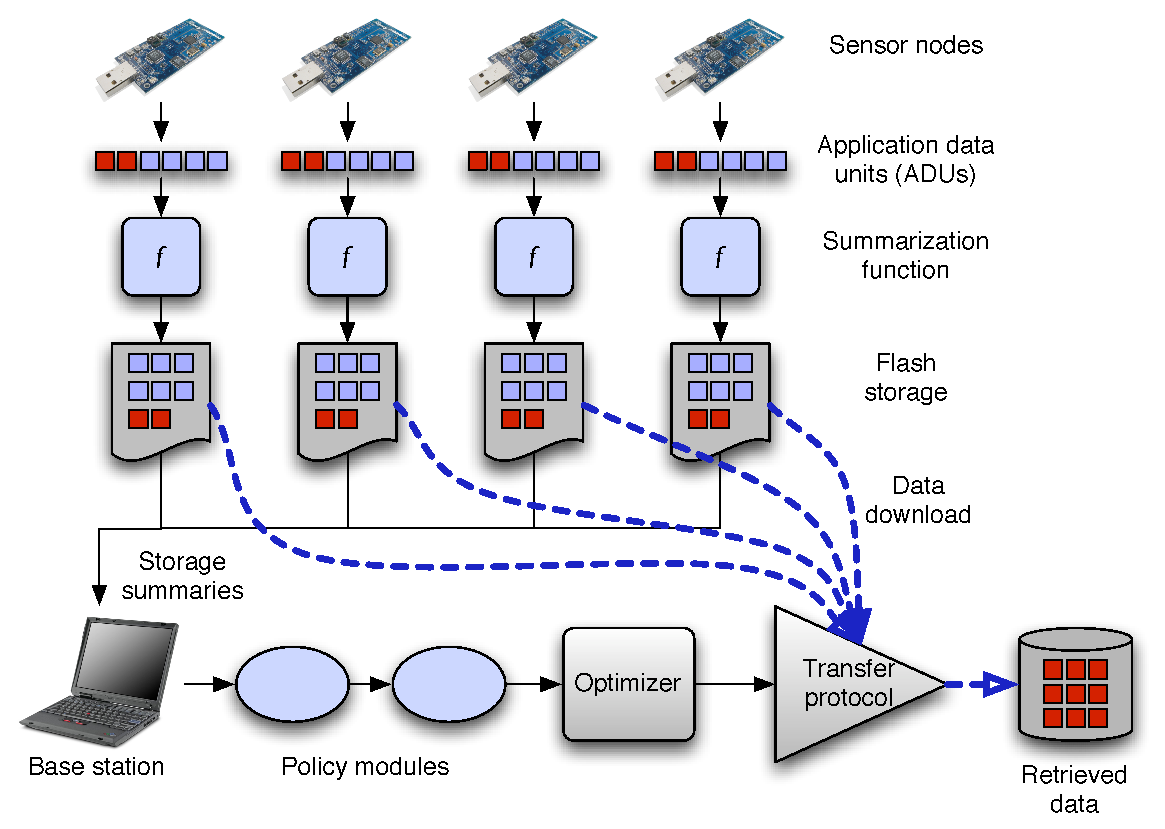
\includegraphics[width=1.0\hsize]{./figs/Sensys2008/2008-lance-architecture.eps}
\end{center}
\caption{{\bf Lance architecture.}
The architecture of both the priority- and utility-driven versions of
Lance is quite similar. The interpretation of the assigned utility values
differs, but the major architectural components are the same.}
\label{fig-lance-architecture}
\end{figure}

Figure~\ref{fig-lance-architecture} provides an overview of the Lance
architecture. Sensor nodes sample sensor data, storing the data to local
flash storage. Each application data unit (ADU) consists of some amount of
raw sensor data, a unique {\em ADU identifier}, and a {\em timestamp}
indicating the time that the first sample in the ADU was sampled. ADU
timestamps can either be based on local clocks at each node, or tied to a
global timebase using a time synchronization protocol such as
FTSP~\cite{ftsp}. The size of an ADU should be chosen to balance the
granularity of data storage and download with the overhead for maintaining
the per-ADU metadata. In the applications we have studied, an ADU stores
several seconds or minutes of sensor data, not an individual sample. ADUs are
stored locally in flash, which is treated as a circular buffer.

Ideally, nodes would be able to compute the value $v_i$ of an ADU locally, as
the data is sampled. However, since the value might depend on factors other
than the ADU's data, such as data computed at other nodes. Lance assigns
values $v_i$ at the base station, based on global knowledge of the state of
the network. However, this requires nodes to communicate some low-bandwidth
information on the ADU contents to the base station.  For this purpose, each
node applies an application-supplied {\em summarization function}, computing
a concise summary $s_i$ of the contents of the ADU as it is sampled.  Nodes
periodically send {\em ADU summary} messages to the base station, providing
information on the ADUs they have sampled, their summaries, timestamps, and
other metadata. As a special case, if a node is able to assign the ADU's
initial value directly, this is used as the summary.

The Lance {\em controller} receives ADU summaries from the network.  The
controller also estimates the download cost $\bar{c}_i$ for each ADU, based
on information on network topology as well as a model of energy consumption
for download operations. The ADU summaries and cost are passed through a
series of {\em policy modules}, which provide application-specific logic to
assign the value $v_i$ to each ADU.  The resulting values are passed to the
Lance {\em download manager} which is responsible for performing downloads,
using a reliable data-collection protocol, such as
Flush~\cite{flush-sensys07}.

\subsection{Cardinal v Ordinal Utilities}

One significant difference between the first and second versions of Lance is
the meaning of the utility values assigned to each ADU.  Utility values
assigned to each ADU are intended to reflect the value of that signal to the
application, with higher utilities indicating more valuable data.  Accurate
and efficient utility assignment -- while a difficult and
application-specific challenge -- is crucial to the Lance approach.

The first version used \textit{ordinal} utilities (or priorities), meaning
that the assigned utilities established an order among available ADUs but did
not reflect the relative importance of one ADU versus another. Given
priorities, an ADU assigned priority 100 can only be assumed to me more
valuable that one assigned an ADU 99. It might be 100 times more valuable. It
might be only 2 times more valuable.  The fact that ordinal utilities produce
a strict ordering and nothing else simplified the policies of the first
system. The storage manager could easily prioritize available flash on each
node, and the download manager simply downloaded the available ADU with the
highest utility, irregardless of the resources necessary to do so. Since
ordinal utilities do not allow the value of an ADU to be weighed against the
cost (in system resources) required to download it, they render the notion of
cost unnecessary.

The second iteration of Lance used \textit{cardinal} utilities, which not
only produce an ordering but also imply relative value between ADUs. So an
ADU assigned utility 100 is assumed to be twice as valuable as one assigned
utility 50. This formulation allows the incorporation of cost into the
optimization framework, as described later in Sect.~\ref{sec-lance}.

\subsection{Utility Functions}

Implicit in Lance is the idea that, when addressing dataset quality, wheat
must be separated from chaff. We rely on a utility function to do so,
irregardless of whether the utility is interpreted as a cardinal or ordinal
one.  In general utility functions can be quite complex, depending not only
on the data acquired at a particular node but also on the distribution of
data across the network, availability of storage, bandwidth, energy and other
resources, and so forth.  To help designers construct complete systems
\textit{without} starting from scratch, Lance attempts to cleanly separate
the \textit{policies} governing how to divide data into interesting and
uninteresting piles from the \textit{mechanisms} governing the collection of
data after the division is performed.

To leverage global knowledge while reducing the resource consumption on each
node, we separate local knowledge from global by effectively diving the
utility assignments between node-specific (the utility calculator that runs
on each node) and network-wide (the policy module chain described in the next
section) components.  The node-level utility calculator operates only based
on inputs available on a single node and must run on a resource-constrained
sensor network node, limiting the amount of computation it can perform.  In
contrast, the network-wide policy modules running on the powered base station
have access to a global view of the network and significantly augmented
resources. As such they can use global, historical and out-of-band
information to further refine the initial utility assignment performed on the
node itself.

Communication between the node-level and network-wide portions of the utility
function is overhead with respect to the application goals, and so a
practical requirement limiting the usage of Lance is keeping the traffic
between these two components to a minimum. The utility functions we have
developed in the context of the volcano application have typically limited
this overhead by having the output of the node-level utility function be a
single scalar value, which can be efficiently transmitted to the base
station.  There is no requirement that the node-level utility function
produce such simple outputs, but it does aid in reducing the overhead
inherent in the utility assignment process.

As a concrete example tying Lance to previous work, the distributed event
detector deployed at Reventador in 2005 could be easily reimplemented in
Lance. The node-level utility calculator uses the ratio of two EWMAs to
assign a binary utility, either one or zero, to each ADU. At the network
level, a policy module aggregates these assignments and, when enough overlap
within a particular time window, it marks that entire segment of data with a
unit utility value (all other time windows receive utility zero). Because
each ``interesting'' set of signals receives the same utility value, Lance
does not distinguish between them and will download them in a LIFO fashion.

\subsection{2007 Deployment}

To evaluate the performance of Lance in a real field setting, we undertook a
one week deployment of eight~sensor nodes at Tungurahua Volcano, Ecuador, in
August~2007. The priority-driven version of Lance was used to manage the
bandwidth resources of the sensor network, as described below. Time and
budget constraints prevented us from deploying a larger network for longer
period of time. Our primary goal was to validate Lance's operation in a field
campaign, as well as to identify challenges that only arise in real
deployments. Our experiences during this deployment led to further
refinements of Lance described in the next section.

\begin{figure}[t!]
\caption{{\bf Download performance during the deployment.}}
\vspace{0.2in}
\begin{center}
\begin{tabular}{lll}
\noalign{\smallskip}
{\bf Node}	& {\bf ADUs downloaded} & {\bf Mean throughput} \\
\noalign{\smallskip}\svhline\noalign{\smallskip}
100 & 311 & 651.0 B/sec \\
101 & 131 & 446.8 B/sec \\
102 & 262 & 445.8 B/sec \\
103 & 292 & 424.4 B/sec \\
104 & 150 & 256.8 B/sec \\
105 & 66 & 453.7 B/sec \\
106 & 20 & 253.4 B/sec \\
\noalign{\smallskip}\svhline\noalign{\smallskip}
{\em Total} & 1232 & 431.5 B/sec \\
\end{tabular}
\end{center}
\label{fig-throughputtable}
\end{figure}

The sensor network was operational for a total of 71~hours, out of which the
Lance download manager ran for a total of 56~hours.  During this time, Lance
successfully downloaded 1232~ADUs, or 77~MB of raw data. An additional
308~downloads failed due to timeout or stale summary information, for an
overall success rate of 80\%.  11012~unique ADU summaries were received from
the network, representing an aggregate of 688~MB of sampled data. Lance
therefore downloaded approximately 11\% of the data produced by the network.
Figure~\ref{fig-throughputtable} summarizes the number of ADUs downloaded
and the mean throughput for each node. 

\subsubsection{RSAM v EWMA Node Level Utility Calculator}
\label{subsubsec-rsamvewma}

The system as initially deployed computed the RSAM~\cite{rsam} (Reduced
Seismic Amplitude Measurement) as the value for each ADU.  This approach was
intended to prioritize data based on the overall level of seismic activity.
We experienced two problems as soon as the system was fielded. First, the
RSAM calculation was sensitive to DC~bias in the seismometer signal, causing
Lance to generally prefer downloading ADUs from one or two nodes (those with
the largest positive bias). We were able to work around this problem using
\textit{policy modules}, described in the next section.

The second problem with the RSAM utility calculator was caused by the
uncharacteristically low level of seismicity at the volcano throughout the
deployment. We observed only about 20~volcano-tectonic earthquakes and {\em
no} clear explosions, whereas the previous week, Tungurahua exhibited dozens
of earthquakes each day. As a result, the RSAM utility calculator was
generally unable to distinguish between actual seismic activity and noise.
Given the low level of volcanic activity, after the first 25~hours of the
deployment we chose to reprogram the network to use a different utility
calculator designed to pick out small earthquakes from background noise.  This
function computes the maximum ratio of two EWMA filters over the seismic
signal; it is similar to that described in~\cite{volcano-osdi06}. Due to code
size limitations on the motes, it was necessary to manually reprogram each
node with the new utility calculator, which took two teams about 4~hours.

We return to the 2007 deployment later in this chapter in two other contexts.
First, we discuss \textit{policy modules}, a useful feature that spanned both
the priority- and utility-driven versions of Lance.  We illustrate their use
with examples from our field deployment. Finally we present the mature,
utility-driven Lance, and also include an evaluation of its performance based
on data collected during our 2007 deployment.

\section{Policy Modules}
\label{sec-policymodules}

Policy modules provide an interface through which applications can tune the
operation of the download manager.  As previously described, along with the
node-level utility assignment they make up the utility function responsible
for providing input to the download manager.  Lance requires that policy
modules be efficient in that they can process the stream of ADU summaries
received from the network in real time. In practice this is not difficult
to accomplish, as the rate of ADU summary reception is modest, and the base
station (typically a PC or laptop) is assumed to have adequate resources.
For example, a 100-node network with an ADU size of 60~sec would receive an
ADU summary every 600~msec. Typical policy modules take a small fraction of
this time to run. 

One of the main benefits of policy modules is that they permit significant
changes to the network's behavior {\em without requiring changes to the
node-level utility assignment}. Changing the latter would typically involve
reprogramming sensor nodes. Based on our experience at Reventador we were
wary of reprogramming the network unless absolutely necessary. Although
systems such as Deluge~\cite{deluge} permit over-the-air reprogramming, any
changes to the sensor node software could result in unexpected failures that
can be very difficult to debug without manual intervention.  On the other
hand, introducing new policy modules at the base station is relatively
straightforward, and can be quickly reversed without risking sensor node
failures. 

\subsection{Example Policy Modules}

Policy modules can be used to encapsulate a wide range of data collection
goals, and make it easy to customize Lance's behavior for specific
applications. While we provide a standard toolkit of general-purpose policy
modules, application developers are free to implement their own modules as
well.  By composing modules in a linear chain, it is easy to implement
various behaviors without requiring a general-purpose ``policy language.'' 

{\bf Priority thresholding:}
{\tt filter} is perhaps the simplest example of a policy module that filters
out ADUs with a utility below a given threshold $T$.  This type of filtering
can be used to force a drop of low-valued data. Conversely, the {\tt boost}
utility module sets the utility for an ADU above a given threshold to a
very high value, ensuring that it will be downloaded next. 

{\bf Priority adjustment and noise removal:} 
Policy modules can be used to remove the effects of noise or correct 
for node-level utility bias, for example, based on poor sensor 
calibration or differences in site response. Moreover, since each node 
computes the initial ADU utility based only on local sensor data, it may be 
necessary to normalize the ADU utilities in order to compare 
utilities across nodes. 

{\tt adjust} adds or subtracts a node-specific offset to each ADU utility
in order to correct for differences in sensor calibration. {\tt smooth}
applies a simple low-pass filter on the raw utility values to remove
spikes caused by spurious sensor noise.
Likewise, {\tt debias} is intended to remove
sensor-specific DC~bias in the utility values assigned by the node's
prioritization function. {\tt debias} computes the median utility
value for a given node over a given time window. It then subtracts
the median from each ADU utility before passing it along to the next
module in the chain. 

Likewise, when a sensor network contains
multiple sensors with varying sensitivity, it is natural to
prioritize data from more sensitive instruments. In cases where networks are
deployed to monitor fixed physical phenomena, it may be desirable to
prioritize data from nodes located close to the phenomena being
observed. The {\tt adjust} module can be used to scale
raw utilities based on a sensor's location, SNR, or other attributes.

{\bf Priority dilation:} 
Another useful policy is to dilate a high (or
low) utility value observed in one ADU across different ADUs sampled
at different times or different nodes. This can be used to achieve
greater spatial or temporal coverage of an interesting signal
observed at one or more nodes. The {\tt timespread} detects ADUs with
a utility above some threshold $T$, and 
assigns the same utility to those ADUs sampled just before and just
after.

Likewise, the {\tt spacespread} module groups ADUs from across multiple
nodes into time windows and assigns the maximum utility value to all
ADUs in that window.  Define a window $W(t,\delta)$ as the set of ADUs
such that $t-\delta \leq t_i \leq t+\delta$ where $t$ represents the
center of the window and $\delta$ the window size. {\tt spacespread}
determines the maximum ADU in the window $p^* = \arg_{i \in W} \max p_i$
and sets $p'_i = p^{*}$ for each ADU in $W$. 

\begin{figure}[t!]
\begin{center}
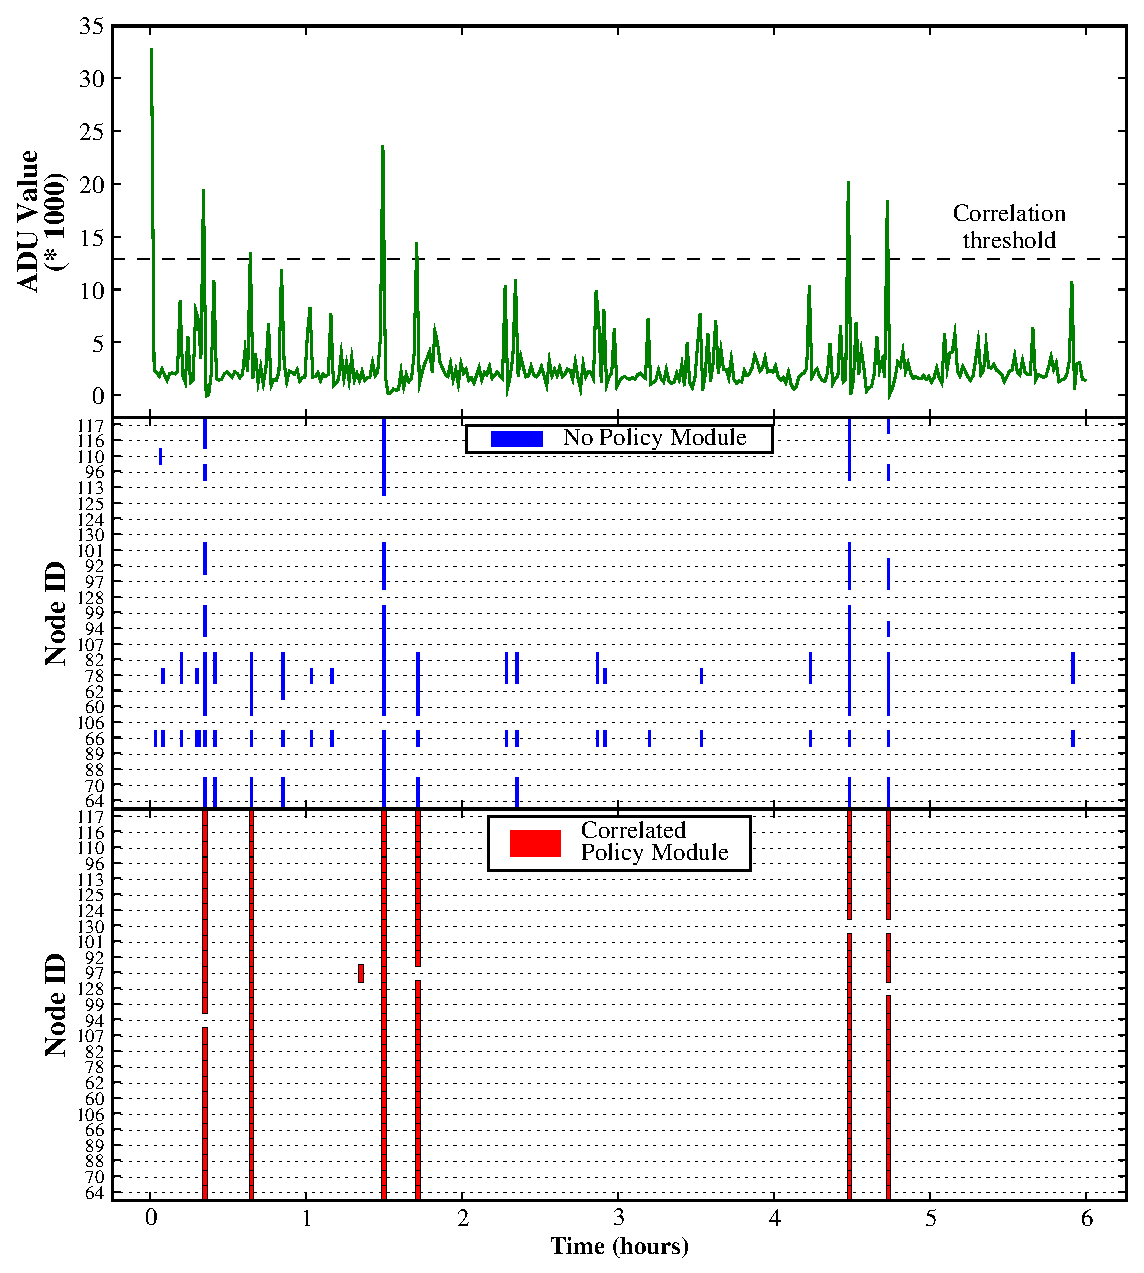
\includegraphics[width=1.0\hsize]{./figs/Sensys2008/2008-policy-module-usage.eps}
\end{center}
\caption{{\bf Usage of policy modules to affect download distribution.} 
Here we illustrate the use of policy modules. The graph compares the download
behavior of the system with and without a policy module chain which assigns
greater values to ADUs corresponding to correlated seismic activity.  The
graph is colored at a particular timestamp and node ID if we downloaded that
signal from that node. The top graph shows the ADU values over time, with the
threshold for the \texttt{filter} component of the policy module chain
indicated.}
\label{fig-policy-module-usage}
\end{figure}


{\bf Correlated event detection:}
The {\tt correlated} module is used to 
select for ADUs that appear to represent a correlated
event observed across the entire sensor network. 
{\tt correlated} counts the number of ADUs within a time window
$W(t,\delta)$ with a nonzero utility value.
If at least $k$ ADUs meet this criterion, we assume that there is 
a correlated stimulus, and the utility values for all ADUs in 
the set are passed through.  Otherwise, we filter out the ADUs in 
the window by setting $p'_i = 0$ for each ADU in $W$.

As an example of composing policy modules to implement an interesting
behavior, consider the chain \[
\mathit{filter}(T)\rightarrow\mathit{correlated}(k)\rightarrow\mathit{spacespread}
\] This policy filters incoming utilities, rejects time-correlated sets with
fewer than $k$ ADUs above the threshold, and assigns the max utility across
the set to all ADUs. This can be useful in systems that wish to perform
collection of time-correlated data, but avoid spurious high-utility data from
just a few nodes.  This policy is equivalent to the volcano earthquake
detector used in our previous work~\cite{volcano-osdi06}, expressed as a
simple policy module chain, and demonstrates, as mentioned in the previous
section, that our distributed event detector can be reimplemented as a Lance
utility function with both node- and network-level components.

\subsection{Evaluation and Use at Tungurahua}
\label{subsec-policymoduleuse}

We evaluated the usefulness of the policy module architecture through testbed
experiments, as well as during our field deployment in 2007.  For the testbed
experiment, we use a distribution of ADU data values based on a 6-hour
seismic trace collected at Reventador Volcano, Ecuador in
2005~\cite{volcano-osdi06}. The raw seismic data is divided into ADUs of 36
KB and ADU values $v_i$ are assigned by computing the ratio of two
EWMA~filters on the data, which assigns greater value to ADUs that contain
earthquakes. For each node in a 25 node topology, the ADU values from the
seismic trace are attenuated based on a hypothetical signal source and
assigned to each of the 25 nodes based on their location with respect to the
signal source. We then enable a policy module chain that assigns higher
priority to ADUs that correspond to correlated seismic activity across the
network.

Figure~\ref{fig-policy-module-usage} shows the result of this experiment
running on the MoteLab testbed. The upper portion of the figure shows the ADU
values over time; the middle portion, the set of ADUs downloaded by the
system with no policy modules in use; and the lower portion, the ADUs
downloaded with the policy module chain in use.  As the figure shows, the
policy modules cause the network to prefer correlated seismic events and
download an ADU from all nodes in the network when such an event is detected.
Gaps in the set of ADUs downloaded are due to download timeouts. In one case,
a single ADU is downloaded spuriously due to an incorrect value being
reported by that node to the base station. This use of policy modules shows
the drastic change in the system behavior that is affected without
programming the sensor nodes themselves.

Our deployment at Tungurahua Volcano allowed us to evaluate the ability to
change download policies at the base station without reprogramming nodes, one
of the significant advantages policy modules provide.  As described in
Sect.~\ref{subsubsec-rsamvewma}, the RSAM utility calculator initially
deployed at Tungurahua was sensitive to DC bias, which caused Lance to
continuously download signals from one or two nodes with large DC biases.

\begin{figure}[t!]
\begin{center}
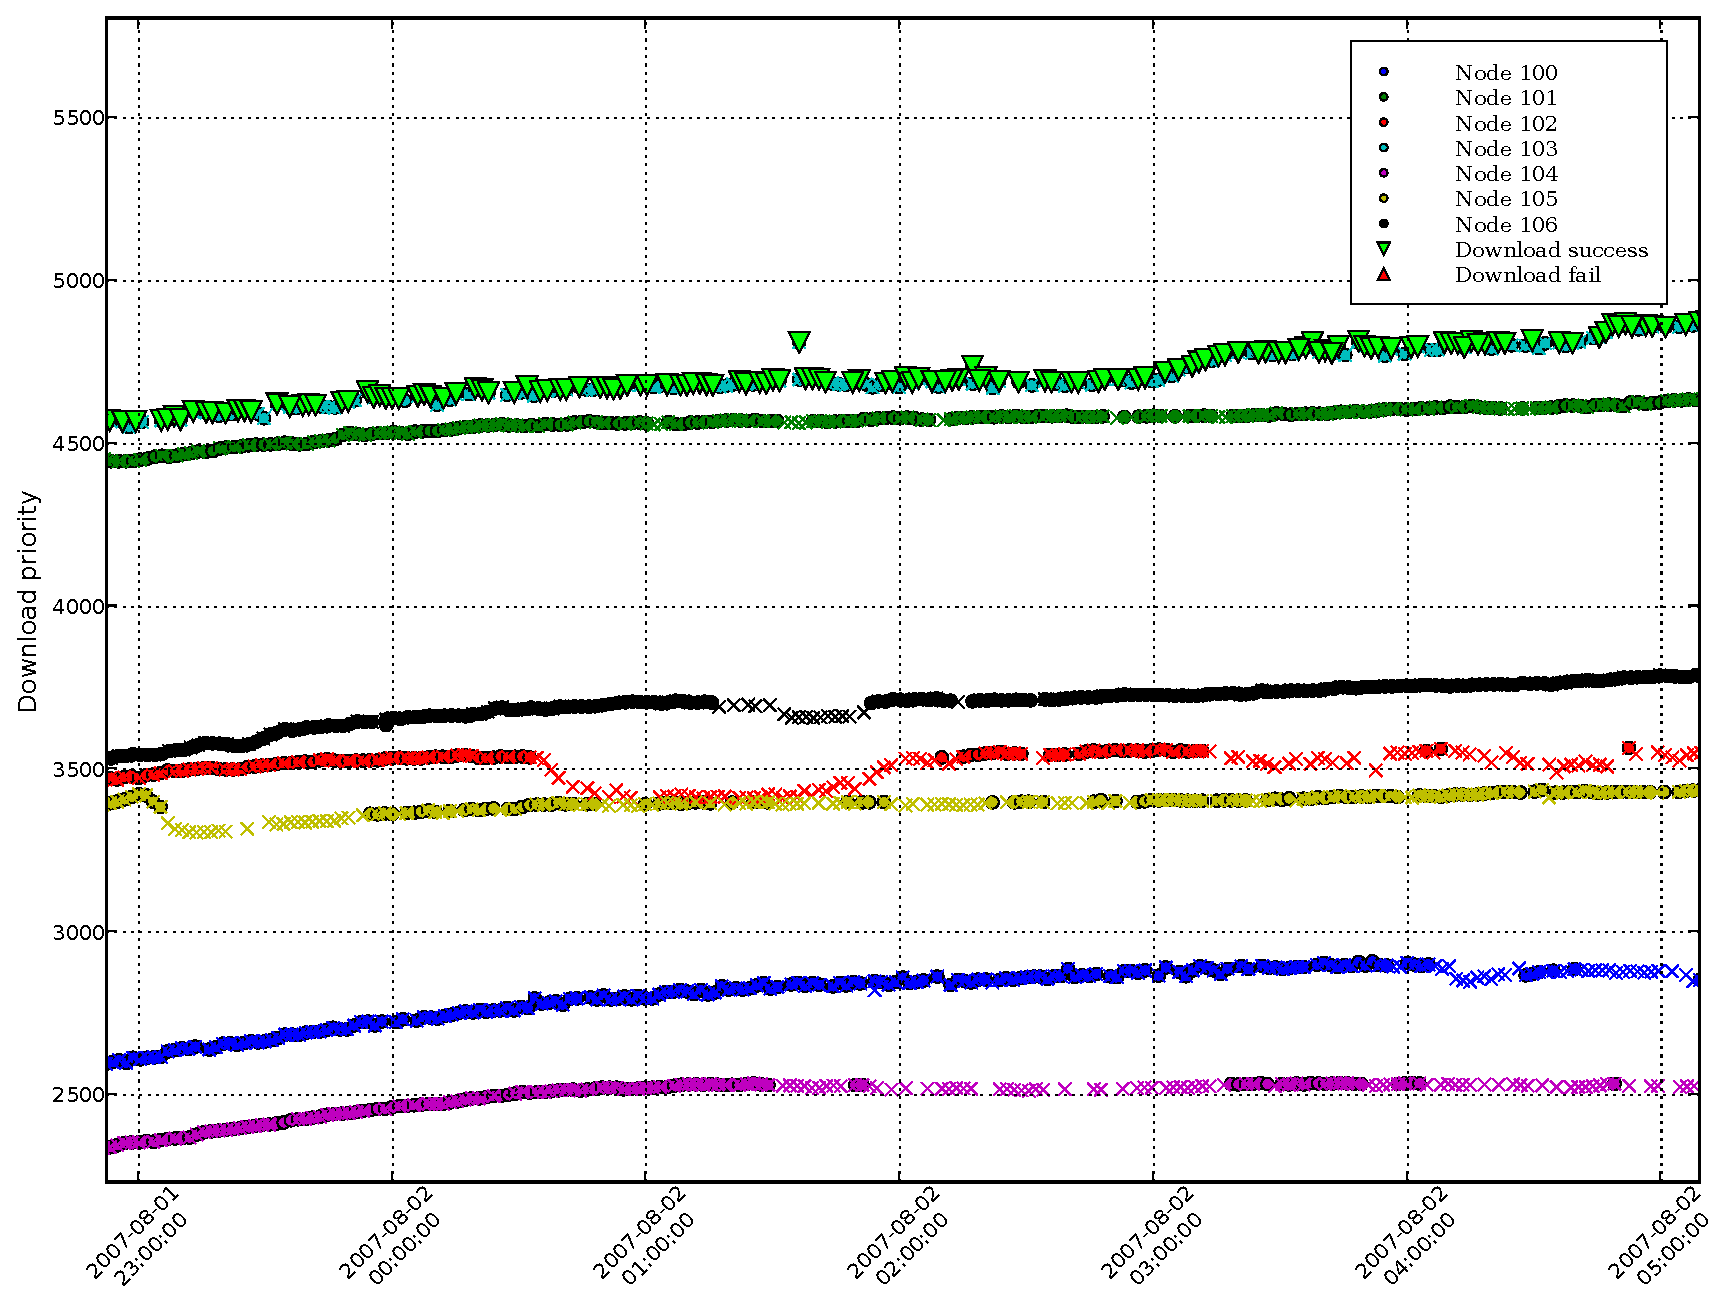
\includegraphics[width=0.7\hsize]{./figs/Sensys2008/2008-downloads-pre-median-filter.eps}\\
\textbf{(a)}\\
\includegraphics[width=0.7\hsize]{./figs/Sensys2008/2008-downloads-post-median-filter.eps}\\
\textbf{(b)}
\end{center}
\caption{{\bf Effect of DC bias on RSAM summarization function.}
Each point represents the ADU value received at the base station, and the
triangles indicate those ADUs that were downloaded by Lance. In \textbf{a},
because nodes' RSAM values are offset significantly from each other, Lance
prefers downloading from the node with the largest positive bias. However,
\textbf{b} shows what happens after applying a simple debiasing policy module
at the base station. This filter removes the DC bias causing Lance to
download from multiple nodes.}
\label{fig-downloads-median-filter}
\end{figure}

This problem was easily corrected, without any node software changes, by
introducing a policy module at the base station to process the raw RSAM
values received from each node and filter out the DC~bias. This was achieved
by computing the median RSAM value over each 30-minute window of raw RSAM
values on each node, and subtracting the median from the RSAM.
Figure~\ref{fig-downloads-median-filter} shows the result of the application
of the filter, with the debiasing effect clearly visible. The ability to
change and correct download behavior from the base station without modifying
sensor node code proved extremely useful in this case, particularly in that
it permitted the rapid iteration necessary to properly craft the appropriate
filter.

\section{Optimizing for Energy and Bandwidth Usage}
\label{sec-lance}
\label{sec-utilitylance}

After completing our 2007 deployment at Tungurahua we rearchitected
our original Lance system and shifted its focus. Instead of optimizing for
storage and bandwidth, we instead chose to optimize primarily for energy,
with bandwidth as a secondary concern. Several changes to the hardware and
software environment explain this shift in emphasis.

First, storage management began to seem less pressing as the promise of
sensor network nodes with large attached flash memories seemed to be becoming
a reality.  The TMote Sky deployed at Reventador had only 1~Mbit of flash,
meaning we could only store around 20~min of signal (from two channels,
24~bits per sample at 100~Hz). In contrast, the SHIMMER mote developed for
medical monitoring can be fitted with a flash card allowing it to store as
much as 2~GB of data, meaning that deployed in support of the volcano
application it could conceivable store over 41~\textit{days} of
full-resolution sampled data (assuming 2 data channels sampled at 100~Hz with
3~bytes per sample).  The idea behind managing storage was that it was
necessary in order to preserve the highest-utility ADUs until the network
controller would get around to downloading them. Once storage sizes swelled
it seemed like a simple FIFO storage policy would allow plenty of time for
interesting data to be downloaded.

Second, support for radio duty cycling entered the TinyOS tree and began to
be used by our group. This shifted our focus from thinking about bandwidth as
a constraint to thinking about the \textit{energy} associated with operating
the radio in order to download data as a constraint. In contrast to the early
Lance system, which deployed a ``greedy'' download manager which strove to
download as much data from the network as possible, once the radio could be
easily disabled when not in use it became natural to want to consider the
cost of downloading signals and not necessarily run the downloads in a greedy
fashion. 

\subsection{Refocusing on Energy Usage}

Shifting the system's concern to energy usage required several changes to the
Lance architecture: a move from ordinal to cardinal utilities, and the
development of a cost model.

Replacing the ordinal utilities with cardinal ones allowed us to compare the
relative value of different ``baskets'' of ADUs in a meaningful way. Two
ADUs, each with a utility of 50 were considered equivalent to the application
as a single one with utility 100.  This meant that instead of simply
downloading the highest-utility ADU available in the network at a given
moment, we needed a way of determining which was the best ADU in terms of
both the value but also the system's ability to extract it.

Given our high data rates, we were already restricted by bandwidth alone to
downloading only a portion of all of the data sampled by every node in the
network.  Once we began using LPL to duty cycle the radio extracting data
also had an impact on energy consumption as well, and so achieving a given
target lifetime could be accomplished by downloading data at slower rates
allowing node radios to be powered off when not in use.  Either bandwidth or
energy could have driven the cost model, but given the dependence of energy
consumption on bandwidth usage (and lack of a similar relationship in the
other direction) we chose to represent the cost necessary to download an ADU
as the \textit{energy} required to retrieve it.

Compared with our original ordinal utility efforts, the new version of Lance
contributed several ideas. First was a way of estimating, a priori,
the energy necessary to extract an ADU from the network. This was necessary
so that both the cost and value of each ADU could be considered before
download decisions were made. For value, we leverage the same two-part
utility-assignment framework described earlier.  The cost estimation
component is described below.

In addition, once the cost and value had been assigned to each ADU, the
problem of deciding which to download can be framed as an optimization
problem. We described a way of producing an optimality bound by mapping an
offline version of this problem to a well-studied optimization problem, and
use this optimality bound to evaluate several online algorithms suitable for
real-time decision making. These contributions are also described in further
detail below.

\subsection{Cost Estimation}
\label{subsec-costassignment}

Each ADU has an associated cost $\bar{c}_i$ that represents the energy
requirement to download the ADU from the network.  $\bar{c}_i$ is a vector
$\{ c_i^1, c_i^2, \ldots, c_i^n \}$ where $c_i^j$ represents the estimated
energy expenditure of node $j$ when ADU $i$ is retrieved. The key idea is
that we explicitly model both the energy cost for downloading the ADU from
its ``host'' node $n_i$ and the energy cost for each node along the
routing path from $n_i$ to the base station which must forward packets during
the transfer. In addition, we also model the energy cost to nodes that
overhear transmissions by nodes participating in the transfer.  This energy
cost on intermediate nodes is non-negligible, since reliable transfer
protocols involve a potentially large number of retransmission. However, the
overhearing cost is typically small, since modern low-power MAC protocols
quickly return to sleep when overhearing transmissions to another node.  The
cost vector $\bar{c}_i$ therefore depends on the network topology.

Lance estimates the download energy cost vector $\bar{c}_i$ for each ADU
sampled by the network.  We assume that nodes are organized into a spanning
tree topology rooted at the base station. The cost is a function of many
factors, including the reliable transport protocol, each node's position in
the routing tree, radio link quality characteristics, and the MAC protocol. 

Given the complex dynamics that can arise during a sensor network's
operation, we opt to use a simple conservative estimate of the energy cost to
download an ADU from a node. Our approach is based on an empirical model that
captures three primitive energy costs involved in downloading an ADU. The
first, $E_d$, represents the energy used to download an ADU from a given node
which includes the energy cost for reading data from flash and sending
multiple radio packets (including any retransmissions) to the next hop in the
routing tree.  The second, $E_r$, represents the energy cost at intermediate
nodes to forward messages during the ADU transfer. The third, $E_o$,
represents the energy cost to nodes that overhear transmissions during a
transfer.  For simplicity, we assume ADUs of fixed size and compute $E_d$,
$E_r$, and $E_o$ based on the time necessary to download an ADU from the
target node.

Using this simple model, we set the elements of the cost vector $\bar{c}_i$ 
as follows. $c_i^n = E_d$ for the node $n$ hosting the ADU, and 
$c_i^m = E_r$ for nodes $m$ along the routing path from
$n$ to the base station. We set $c_i^o = E_o$ for nodes that are
assumed to be within one radio hop of any of the nodes involved in
the transfer. Estimating $\bar{c}_i$ therefore requires
knowledge of the current routing topology. This information 
is readily available: the periodic summary messages, sent to the 
base station by every node, include the node's radio neighbors and 
parent in the routing tree. Cost vectors can be easily recomputed 
whenever the routing topology changes.

To ensure that all nodes meet the lifetime target $L$, Lance models the
energy availability at each node using a token bucket with depth $D$ and fill
rate $C/L$, corresponding to the mean discharge rate.  $D$ is determined by
the target lifetime $L$, the battery capacity $B$ and the background drain
rate $R$.  In general, $D = B - L*R$, so $D$ represents the energy remaining
after the node reserves enough to ensure it can meet its target lifetime at
the background level.

\subsection{Lance Optimizer}
\label{subsec-lanceoptimizer}

The Lance optimizer is responsible for scheduling ADUs for download, based on
knowledge of the set of ADUs currently stored by the network, their
associated values, and costs.  In our design, Lance attempts to download a
single ADU at a time, in order to prevent network congestion, although it may
be possible to download multiple ADUs simultaneously, depending on the
network topology. A download completes either when the entire ADU has been
received or a timeout occurs.

Lance's optimization process attempts to maximize the value of the ADUs
retrieved while adhering to the lifetime target $L$. In essence, we seek a
greedy heuristic approximation of the multidimensional knapsack solution that
would be used by an oracle with complete knowledge of the ADUs sampled by the
network over all time.  The optimizer first excludes ADUs that would involve
nodes without enough energy to perform a download.  That is, if the token
bucket for a given node $m$ has $E(m)$ joules, ADUs for which $E(m) < c_i^m$
are excluded from consideration.  Note that as the bucket fills, the ADU may
become available for download at a later time. We call these ADUs {\em
infeasible}, and the remaining {\em feasible}.

To determine the next ADU to download, the optimizer considers the 
value $v_i$ of each ADU and the its associated cost $\bar{c}_i$.
We consider three {\em scoring functions} that assign a 
download score to each feasible ADU; the ADU with the highest download score
is downloaded next. In the case of ties, an arbitrary ADU is chosen.

The first scoring function, {\em value-only}, simply downloads the feasible
ADU with the highest value $v_i$. Note that {\em value-only} will meet the
network's lifetime target (since only feasible ADUs are considered) but does
not rank ADUs according to cost.  The second scoring function, {\em
cost-total}, assigns the score $\hat{v}_i$ by scaling the value of the ADU by
its total cost: $\hat{v}_i = v_i / \sum_j c_i^j$. The feasible ADU with the
highest score is then downloaded from the network. This approach penalizes
ADUs stored deep in the routing tree, which have a higher overall cost than
those located near the base station. 

The third scoring function, {\em cost-bottleneck}, scales the ADU value $v_i$
by the cost to the node that is an energy bottleneck for downloading this
ADU. That is, let $b$ represent the node with the minimum value of $E(b)$
such that $c_i^b > 0$. {\em cost-bottleneck} sets the score $\hat{v}_i = v_i
/ c_i^b$. The intuition behind this scoring function is that the most
energy-constrained node should be considered when scoring ADUs for download.
We evaluate all three scoring functions in the next section and show that
they yield very different results in terms of spatial distribution and energy
efficiency.

We evaluate each scoring function against an optimal solution calculated by
using knowledge of all future ADUs and solving the multi-dimensional knapsack
problem. Since an online solution is required, this provides an upper bound on
the achievable performance of the online scoring functions.

\subsection{Evaluation and Results}
\label{subsec-evaluationandresults}

Prior work~\cite{lance-sensys08} presents a thorough and detailed evaluation
of Lance on a variety of real and synthetic workloads, evaluated both in
simulation and in experiments on a large sensor network
testbed~\cite{motelab}.  We present a subset of these results here to further
the discussion.

\subsubsection{Simulation and Testbed Experiments}

We began by evaluating Lance using a realistic system simulator which allowed
parameters -- ADU size, distribution of ADU values, network topologies,
download speeds, energy costs and target lifetimes to be easily varied. Our
simulations focus first on evaluating the candidate scoring functions described
above, and secondly on assessing the performance of Lance as the parameters
above are varied.

\begin{figure}[t]
\begin{center}
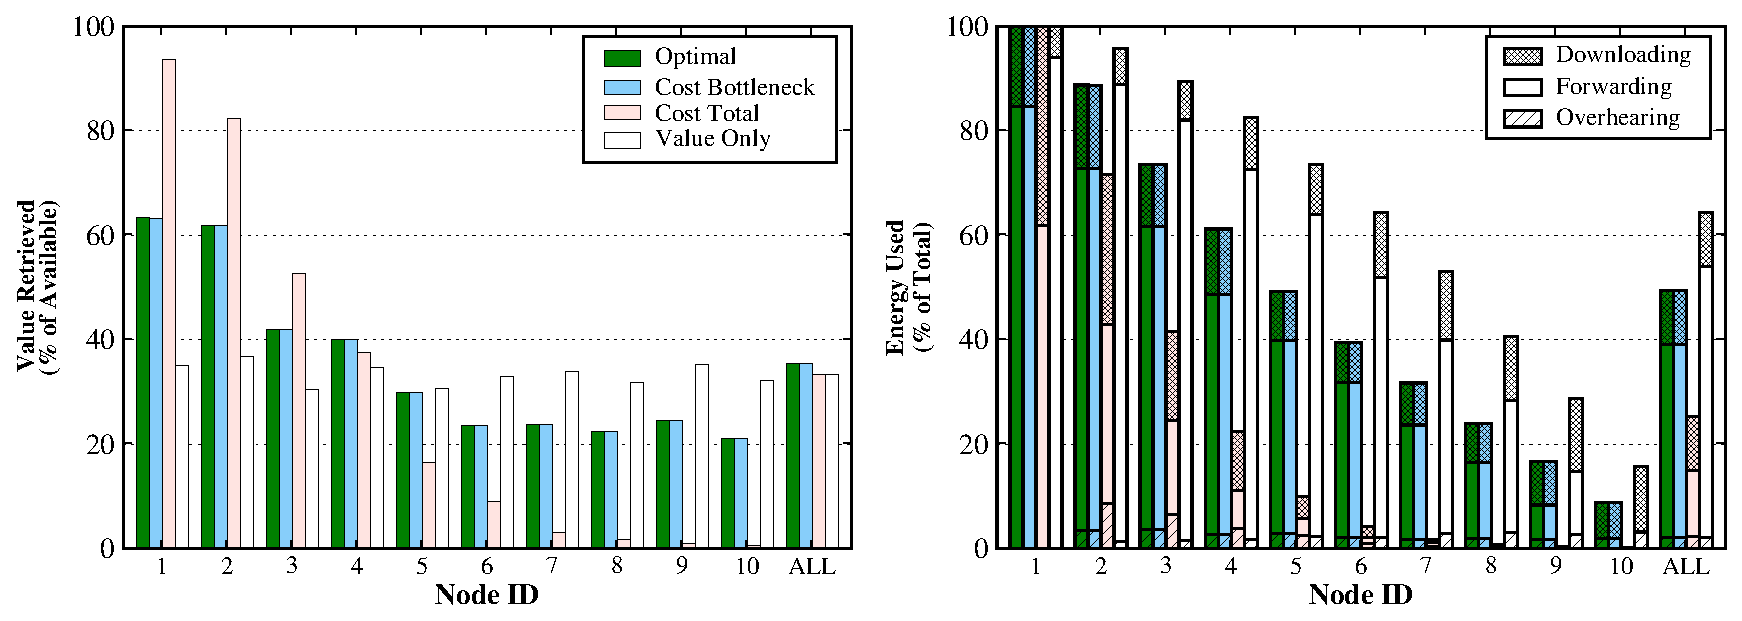
\includegraphics[width=1.0\hsize]{./figs/Sensys2008/2008-lance-linearsimulation.eps}
\end{center}
\caption{{\bf Per-node distribution of ADU value and energy usage for the
linear simulation experiment.} 
The left graph shows the amount of data value downloaded from each node,
while the right graph breaks down the amount of energy used by each node into
the downloading, routing and overhearing components. Node~1 is closest to
the base station.}
\label{fig-lance-linearsimulation}
\end{figure}

Our first simulation experiment used a simple 10-node linear topology.
Figure~\ref{fig-lance-linearsimulation} shows both the performance of each
scoring function against the offline optimal system and a breakdown of the
estimated energy consumed on each node during the simulation. We divide each
node's energy usage into three components: \textit{downloading} energy
consumed by the node when it is transferring one of its own ADUs to the base
station, \textit{forwarding} energy consumed while transferring data upstream
for a downstream node, and \textit{overhearing} energy which accounts for the
small overhearing penalty imposed by the TinyOS LPL implementation on nodes
that overhear (but are not participating in) nearby transfers.

The energy costs for various operations are modeled as follows.  The
background current drain of each node is set to 2~mA, based on empirical
measurements of a TMote~Sky sensor node performing high-data-rate sampling and
storing to flash.  We also measured the current consumption to download an ADU
from a sensor node, and derived the energy costs for downloading ($E_d =
17.6$~mA), routing ($E_r = 16.9$~mA), and overhearing ($E_o = 2$~mA).
Our experiments assume that each node can only overhear its parent in the
routing tree; developing more detailed overhearing models is the subject of
future work.  Computing the components of the cost vector for a particular ADU
is done by multiplying the current consumption by the ADU download time for
each node either downloading, routing, or overhearing the transmission.

Figure~\ref{fig-lance-linearsimulation} confirms the intuition behind the
scoring function behavior.  \emph{value-only} downloads roughly equal value
from each node, but fails to match the optimal performance. \emph{cost-total}
downloads more data from nodes near the sink.  \emph{cost-bottleneck} comes
close to matching the optimal solution, retrieving over 99\% of the value
retrieved by the optimal solution.

\begin{figure}[t]
\caption{{\bf Optimality of different scoring functions.} 
This table summarizes simulation results evaluating the three different
scoring functions.  Results are shown for several different lifetime targets
and value distributions.  {\em cost-bottleneck} out-performs the others in
almost all cases.}
\vspace{0.2in}
\begin{center}
\begin{tabular}{llccc}
\noalign{\smallskip}
& & \multicolumn{3}{c}{Scoring Functions} \\
& & Value & Cost & Cost \\
Distribution & Lifetime & Only & Total & Bottleneck \\
\noalign{\smallskip}\svhline\noalign{\smallskip}
\multirow{3}{*}{Uniform} & 4 months & 62.4\% & 90.5\% & \textbf{93.2\%} \\
& 11 months & 43.4\% & 68.0\% & \textbf{96.9\%} \\
& 18 months & 44.6\% & 49.0\% & \textbf{90.0\%} \\
\noalign{\smallskip}\svhline\noalign{\smallskip}
\multirow{3}{*}{Exponential} & 4 months & 83.9\% & 85.1\% & \textbf{88.0\%}
\\
& 11 months & 70.4\% & 82.0\% & \textbf{93.0\%} \\
& 18 months & 67.2\% & 72.8\% & \textbf{91.2\%} \\
\noalign{\smallskip}\svhline\noalign{\smallskip}
\multirow{3}{*}{Zipfian} & 4 months & 84.7\% & \textbf{91.4\%} & 87.1\% \\
& 11 months & 63.8\% & 91.1\% & \textbf{96.2\%} \\
& 18 months & 53.1\% & 86.9\% & \textbf{93.8\%} \\
\end{tabular}
\end{center}
\label{fig-lancetable}
\end{figure}

To confirm our intuition we ran a set of simulations using a more realistic
25-node tree topology and using a variety of different ADU value
distributions.  We draw ADU values from several distributions in an attempt to
understand Lance's behavior as the properties of the sampled data change.
Three value distributions are used: uniform random, exponentially distributed,
and Zipf with exponent $\alpha = 1$.  We also make use of an ADU value
distribution based on a 6~hour seismic signal collected at Reventador Volcano,
Ecuador in 2005~\cite{volcano-osdi06} for a later experiment.
Table~\ref{fig-lancetable} summarizes the results, showing that the {\em
cost-bottleneck} scoring function outperforms the other two in most cases,
with optimality values between 87.1\% and 96.9\%.  The one exception is the
4-month Zipfian data set, where \emph{cost-total} slightly outperforms
\emph{cost-bottleneck}.

\begin{figure}[t]
\begin{center}
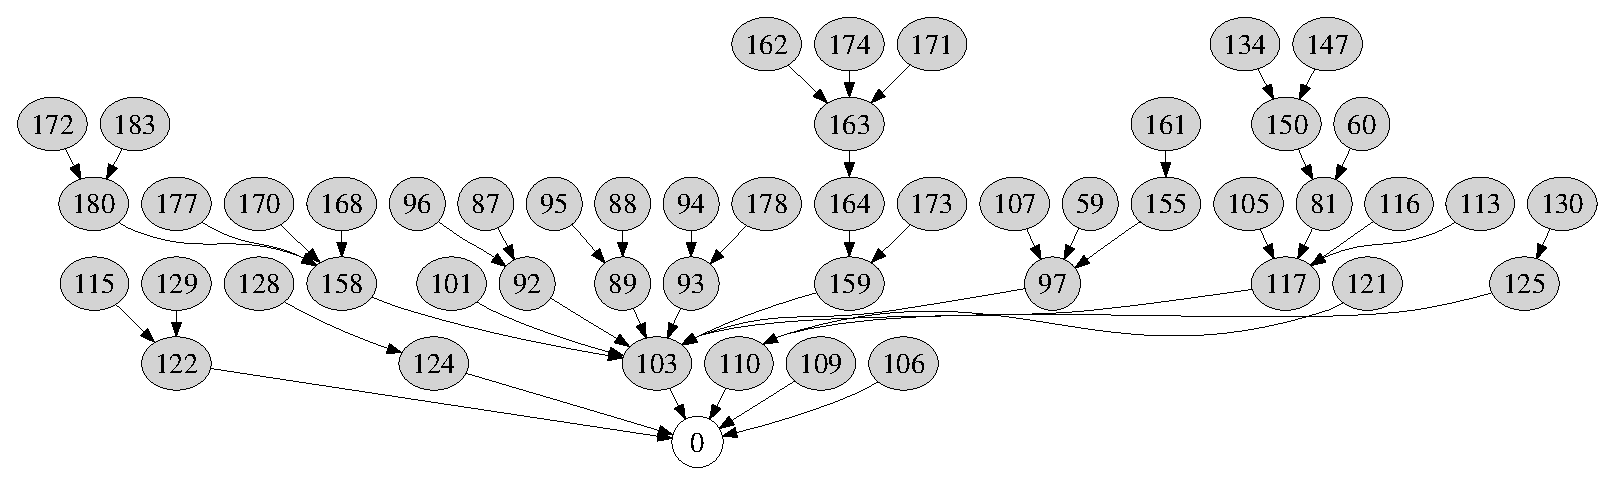
\includegraphics[width=1.0\hsize]{./figs/Sensys2008/2008-lance-testbed-topology.eps}
\end{center}
\caption{{\bf Topology for testbed experiments.} 
This graph shows the 50 node topology used for the testbed experiments shown
in Fig.~\ref{fig-lance-testbed}.}
\label{fig-lance-testbed-topology}
\end{figure}

\begin{figure}[t]
\begin{center}
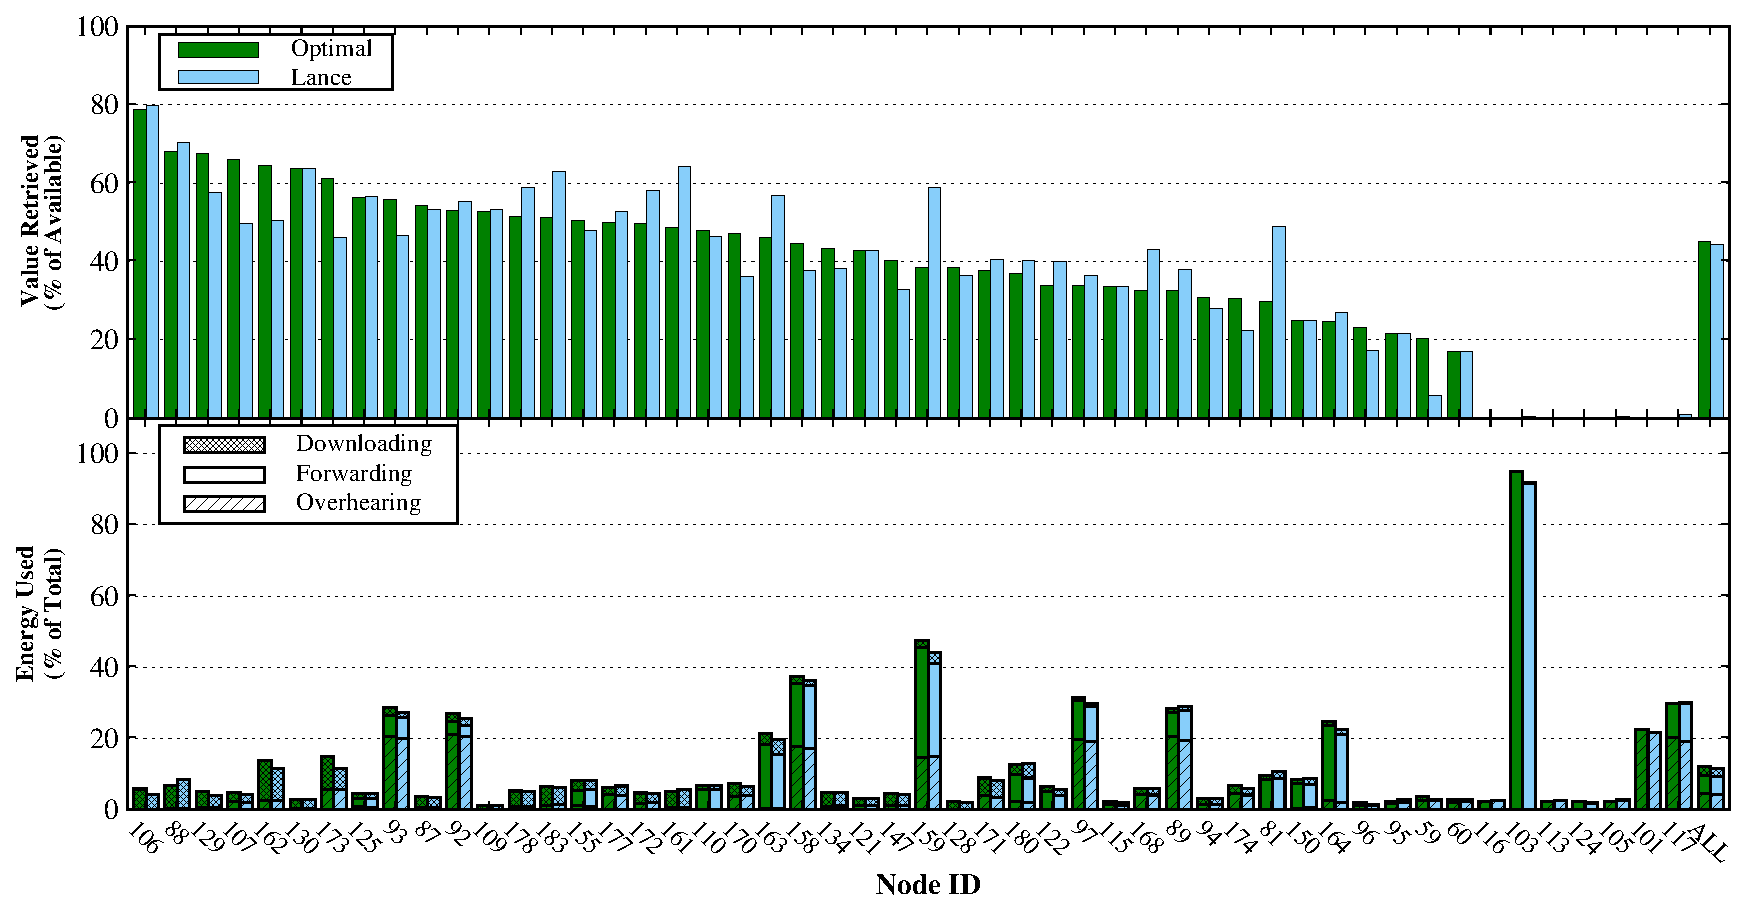
\includegraphics[width=1.0\hsize]{./figs/Sensys2008/2008-lance-testbed.eps}
\end{center}
\caption{{\bf Optimality and energy use in the 50-node testbed experiment.}
Lance achieved near-optimal performance during this 8-hour testbed
experiment, retrieving 98\% of the value obtained by the offline optimal
algorithm.}
\label{fig-lance-testbed}
\end{figure}

We also ran Lance on our MoteLab~\cite{motelab} Wireless Sensor Network
Testbed, in a 50-node configurations shown in
Fig.~\ref{fig-lance-testbed-topology}. These experiments stress the system in a
realistic setting subject to radio interference and congestion, and exercise
the multihop routing protocol, Fetch reliable data-collection protocol, and
ADU summary traffic generated by the nodes. For these experiments, we
injected artificial ADU values directly into each node rather than relying on
the nodes sampling real sensor data; this approach allows us to perform
repeatable experiments that explore a wider range of ADU value distributions.
We use the \emph{cost-bottleneck} scoring function. 

Figure~\ref{fig-lance-testbed} shows the results of a 50-node testbed
experiment using a Zipfian data distribution and a target lifetime of
6~months.  The upper portion of the figure shows the amount of data value
obtained by Lance from each node, compared to the optimal solution (which was
computed offline). Nodes are sorted by decreasing optimal value. As the
figure shows, Lance achieves very close to the optimal solution, with an
optimality of 98\% overall.  In some cases, Lance incorrectly downloads more
data from some nodes and less data from others; this is due to the inherent
limitations of an online solution that cannot foresee future ADU values.  The
lower portion of the figure shows the energy breakdown for each node with
downloading, forwarding, and overhearing costs shown.  Some nodes consume
more than others because of their location in the routing tree. For example,
node~103 in uses a great deal of energy for routing packets as it is one hop
from the base station, although no ADUs are ever downloaded from that node.

\subsubsection{2007 Deployment Analysis}

While the earlier, priority-based version of Lance was used to drive our 2007
deployment at Tungurahua, we were still able to analyze this system's
performance using utility-based metrics.  To evaluate Lance's behavior with
respect to an ``optimal'' system, we took the 8483~RSAM summaries received
during a 16-hour period when the debiasing filter (see
Sect.~\ref{subsec-policymoduleuse}) was enabled. Using this
information, we compute the set of ADUs that the optimal system would have
downloaded, with complete knowledge of all ADUs but limited to the same time
duration the original network was operating.  We assume the download
throughput for a given node is always the mean throughput for that node
observed during the deployment (see Fig.~\ref{fig-throughputtable}). This
calculation ignores energy constraints because the deployed system did not
consider energy costs.

An optimal system would have downloaded 392~out of the~8483 ADUs,
whereas the actual system downloaded 418~ADUs during this 
time.\footnote{The optimal system would download fewer ADUs 
than the real system due to the variation in the throughput to each 
node: the optimal system would download more ADUs from nodes 
with lower throughput, thereby limiting the total number of ADUs it could
download.} The total value of ADUs downloaded by the optimal system 
is 10678, whereas the value of the actual network was 10629, for an
optimality of 99.5\%. Lance did an exceptional job of extracting the
highest-value data from the network using our online heuristic
algorithm.

We can perform a similar analysis during the period of time during which the
network was using the EWMA-based summarization function. As with the
RSAM-based summarization function, we estimate the optimal set of ADUs that an
oracle would have downloaded. During a 25-hour period, the network reported
11012~unique ADU summaries. An optimal system would have downloaded 554 ADUs
with total value 577377.  The actual network downloaded 518~ADUs with a value
of 539115, for an optimality of 93.3\%. 

As a final evaluation metric, we wish to consider how well Lance, configured
in this manner, was able to download seismic signals representing earthquakes.
Given the low level of volcanic activity, it turns out that most of the ADUs
downloaded by Lance contain no discernible seismic signal. In fact, upon
manual inspection of the 518~ADUs downloaded during this period, we identified
only 20~ADUs showing a clear earthquake signal, corresponding to only
9~separate seismic events.  Note that we did {\em not} configure Lance to
explicitly download correlated earthquakes by using an appropriate policy
module (described in Sect.~\ref{sec-policymodules}), so we would not expect
a high degree of coverage for the same event across multiple nodes.

\begin{figure}[t]
\begin{center}
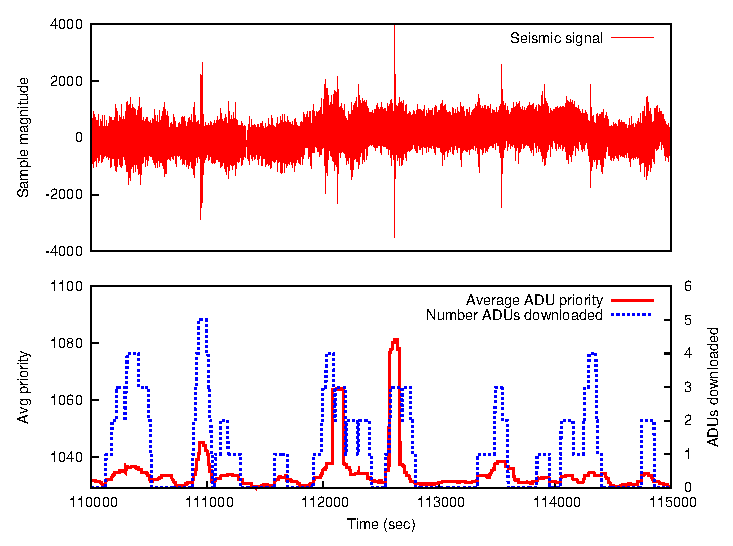
\includegraphics[width=1.0\hsize]{./figs/Sensys2008/2008-lance-download-behavior.eps}
\end{center}
\caption{{\bf Lance download behavior overlaid with average ADU value.}
The top plot shows the continuous seismic signal collected by a single node.
The lower plot shows the average value of ADUs and the number of ADUs
downloaded for each window.}
\label{fig-lance-download-behavior}
\end{figure}

Figure~\ref{fig-lance-download-behavior} shows the behavior of Lance during a
representative 83-minute period. In the figure, we have broken time into
windows of one-half an ADU duration (55~sec in this case), and computed the
mean ADU value as well as the number of downloaded ADUs that overlap each time
window. As the data shows, elevated seismic activity is well-correlated with
an increase in the ADU value from across the network, as well as the number of
downloaded ADUs.  Moreover, the few cases of clear seismic activity in the
trace (at times 111000, 112700, and so forth) tend to have more ADUs
downloaded. Of the 9~separate seismic events, a total of 27~ADUs were
downloaded, representing a per-event ``coverage'' of 3~ADUs per event.  This
represents just under half of the 7~nodes participating in the network.


\subsubsection{Results Summary}

To summarize the results, we found that the cost
bottleneck scoring function allows Lance to approach optimal performance
across a variety of network sizes, bandwidth distributions and target
lifetimes.  By directing scarce energy resources towards the most valuable
data, the overall efficiency of the network considered as a whole can be
significantly increased.

\section{Conclusions}
\label{idea-sec-conclusions}


\acknowledgement{
The authors would like to acknowledge those who helped make this project
possible. Professors Jeff Johnson (New Mexico Tech) and Jonathan Lees
(University of North Carolina), our seismology collaborators, made the entire
endeavor happen, schooling computer scientists in the fine art of
volcanologic research and providing invaluable assistance with the design and
deployment of each of our systems. Mario Ruiz (IGEPN) and Omar Marcillo (New
Mexico Tech) provided additional domain science and deployment assistance.
Harvard students Konrad Lorincz, Pat Swieskowski and Stephen Dawson-Haggerty
helped design and implement the sensor network systems we deployed.
Researchers, staff and students at the Inst\'{i}tuto Geofisico, Escuela
Polit\'{e}cnica Nacional (IGEPN) in Ecuador provided essential ground support
during each of our deployments. Finally, Jim MacArthur and William Walker at
the Harvard School of Engineering and Applied Sciences Circuit Lab aided
significantly in the design and construction of our interface board and
enclosures.

}

\bibliographystyle{spmpsci}
\bibliography{volcanochapter}

\end{document}
